% template.tex, a sample LaTeX manuscript prepared for the Journal of Computer Science and Cybernetics. 
% Run LaTeX on this file twice for proper section numbers.
% A '%' causes LaTeX to ignore remaining text on the line
\input TinLatex_review.tex
\usepackage{subcaption} 
\newcounter{algorithm}
\renewcommand{\thealgorithm}{Algorithm~\arabic{algorithm}}
\begin{document}           % End of preamble and beginning of text.
%------------------------------------------
% Redefine "plain" pagestyle
\makeatletter	   % `@' is now a normal "letter' for LaTeX
\setcounter{page}{1}
\renewcommand{\ps@plain}{%
%\renewcommand{\@oddhead}{\small\hfill\itsl{T\ang p ch\is\ Tin h\ong c v\ah\ \DD i\eeh u khi\eehoi n h\ong c, T.25, S.1 (2009), 1--}}
\renewcommand{\@oddhead}{\hfill\begin{tabular}{r}
\small{\emph{Journal of Computer Science and Cybernetics, V.xx, N.xx (2026), 1--}} \\
\footnotesize{DOI:~10.15625/1813-9663/xx/x/xxxx}
\end{tabular}
}

%\hfil\textrm{\thepage}}% 
    \renewcommand{\@evenhead}{\@oddhead}%
    \renewcommand{\@oddfoot}{\small\hfill{\copyright\ 2026 Vietnam  Academy of Science \& Technology}}% empty footer
    \renewcommand{\@evenfoot}{\@oddfoot}}
    \makeatother     % `@' is restored as a "non-letter" character
    

%%%%%%%%%%%%%%%%%%%%%%%%
%Title & Authors
%%%%%%%%%%%%%%%%%%%%%%%%

%=========================================================================
% \supertitle{Review Paper}
\title{Hybrid UAV Trajectory Optimization via Search Initialization and Quantum-Inspired Evolutionary Algorithms}

\author{
    Huu Phu Le$^{1}$, 
    Phuc Hao Do$^{2}$, 
    Nang Hung Van Nguyen$^{1}$
    \thanks{$^{1}$ University of Science and Technology - The University of Danang, Da Nang, Vietnam; phule9225@gmail.com, nguyenvan@dut.udn.vn; Corresponding author: nguyenvan@dut.udn.vn}
    \thanks{$^{2}$ Danang Architecture University, Da Nang, Vietnam; haodp@dau.edu.vn}
}

\maketitle

% Phần Running Head (tên tác giả xuất hiện ở đầu các trang sau)
\markboth{\footnotesize \chu Huu Phu Le, Phuc Hao Do, Nang Hung Van Nguyen}
{\footnotesize \chu Hybrid UAV Trajectory Optimization via QIEA}

%=========================================================================
\begin{abstract}
Efficient trajectory planning for UAVs in airspaces with multiple No-Fly Zones (NFZs) is a critical multi-objective optimization challenge involving the simultaneous minimization of path length and waypoint count. Classical grid-based search algorithms (A*, Dijkstra, Theta*) guarantee feasibility but produce sub-optimal paths constrained by discretization, while standalone metaheuristics struggle to establish collision-free solutions reliably. To address this dichotomy, we propose a Hybrid Trajectory Optimization Framework operating in two phases: \textbf{Phase 1} employs classical search to rapidly generate a feasible initial path, and \textbf{Phase 2} applies a \textbf{Quantum-Inspired Evolutionary Algorithm (QIEA)} to refine waypoint coordinates in continuous space. QIEA exploits quantum superposition principles for superior global exploration, effectively decoupling the trajectory from the underlying grid structure. Comparative simulations on 50×50 grid environments demonstrate that the hybrid approach achieves over 30\% reduction in path length and drastically reduces waypoint count (e.g., from 35 to 7–8), confirming QIEA as a highly effective post-processing tool for offline UAV mission planning.

\keywords{UAV Trajectory, Hybrid Optimization, Path Refinement, Quantum-Inspired Computing, Metaheuristics, Multi-Objective Optimization, No-Fly Zones.}
\end{abstract}

%%%%%%%%%%%%%%%%%%%%%%%%
%Main text
%%%%%%%%%%%%%%%%%%%%%%%%

%=========================================================================
\section{INTRODUCTION}


% Đoạn 1: Tầm quan trọng của UAV và lập kế hoạch quỹ đạo trong môi trường phức tạp.
Unmanned Aerial Vehicles (UAVs) have evolved from niche military applications into versatile platforms indispensable across numerous civilian sectors, including disaster response, infrastructure monitoring, precision agriculture, and commercial delivery services \cite{ref1}, \cite{ref2}. Central to the effective deployment of UAVs is the field of trajectory planning, which involves generating a safe, collision-free path from a starting point to a destination. This task becomes significantly challenging in complex and restricted airspaces, such as urban environments or areas characterized by numerous Static No-Fly Zones (\textbf{NFZs}), where avoiding obstacles and adhering to flight regulations are paramount constraints. Efficient trajectory planning is crucial for maximizing mission success while minimizing operational risks.


% Đoạn 2: Công thức hóa bài toán: Tối ưu đa mục tiêu (Length và Smoothness).
The core challenge in modern UAV navigation lies in solving the trajectory planning problem as a \textbf{Multi-Objective Optimization (MOO)} task, where several conflicting performance criteria must be simultaneously minimized \cite{ref3}. The two most critical objectives often include minimizing the \textbf{Total Path Length} to reduce flight time and conserve fuel/battery life, and maximizing \textbf{Path Smoothness}, typically quantified by minimizing the number of unnecessary Waypoints (WP) or sharp turning angles \cite{ref4}. A rugged, non-smooth path (high Waypoints) requires frequent adjustments to speed and orientation, leading to increased energy consumption and reduced mechanical longevity of the UAV system. Therefore, a robust planning algorithm must strike an optimal balance between path length and smoothness while strictly adhering to non-collision constraints with NFZs.


% Đoạn 3: Hạn chế của thuật toán tìm kiếm cổ điển (A*, Dijkstra) và Theta*.
Traditional path planning approaches, such as Dijkstra's Algorithm and the $A^{*}$ search algorithm, are widely used due to their computational efficiency and guarantee of optimality on a discrete grid map \cite{ref5}. However, these grid-based methods are constrained by their discretization, often resulting in "stair-step" paths characterized by high Waypoint counts and limited smoothness. These paths, despite being optimal within the grid structure, are sub-optimal in the continuous physical space, translating to poor flight performance in reality \cite{ref6}. Algorithms like $Theta^{*}$ attempt to address this by allowing line-of-sight paths between non-adjacent grid nodes, significantly reducing the number of Waypoints \cite{ref7}. Nevertheless, even $Theta^{*}$ paths are often confined to the edges or nodes found by the initial search, preventing them from achieving true spatial optimality and continuous refinement.

% Đoạn 4: Giới thiệu Thuật toán Lai (Hybrid Approach) và QIEA Refinement.
To overcome the inherent limitations of pure search algorithms while mitigating the slow convergence typical of standalone metaheuristics, we propose a novel \textbf{Hybrid Optimization Framework}. This framework leverages the speed and guarantee of feasibility provided by classical search algorithms (A*, Theta*, Dijkstra) to generate an initial, collision-free trajectory. This initial path is then fed into a \textbf{Quantum-Inspired Evolutionary Algorithm (QIEA)} for detailed refinement \cite{ref8}. QIEA, inspired by quantum computing principles such as superposition and quantum rotation gates \cite{ref9}, possesses superior exploration capabilities and diversity maintenance compared to standard evolutionary algorithms \cite{ref10}. Our central hypothesis is that by applying QIEA to refine the coordinates of the initial Waypoints in continuous space, the hybrid method can efficiently decouple the optimization process from the underlying grid structure, leading to significantly shorter and smoother paths.


% Đoạn 5: Liệt kê các đóng góp chính (Contributions).
The main contributions of this work are summarized as follows:
\begin{itemize}
    \item We formulate the UAV trajectory planning in environments with non-uniform NFZs as a multi-objective optimization problem, focusing on minimizing Path Length and Waypoints (maximizing smoothness).
    \item We propose a two-phase Hybrid Trajectory Refinement Algorithm that integrates classical search methods (A*, Theta*, Dijkstra) for initial path generation with a QIEA for subsequent continuous-space optimization.
    \item We demonstrate that the QIEA component functions effectively as a powerful post-processing smoothing and optimization tool, resulting in path quality metrics (\textit{Length} and \textit{Waypoints}) that significantly outperform the standalone baseline algorithms.
    \item We conduct comprehensive comparative experiments validating the effectiveness of the proposed hybrid approaches across various search initializations.
\end{itemize}


The implementation code and simulation environment used to generate the results presented in this paper are publicly available at: \url{https://github.com/lephus/FJCAI-2026_uav-qiea-hybrid-optimizer/}.

The remainder of this paper is organized as follows. Section~\ref{sec:related_work} reviews related work. Section~\ref{sec:problem_formulation} details the problem formulation. Section~\ref{sec:proposed_method} presents the proposed hybrid QIEA methodology. Section~\ref{sec:experiments} analyzes the experimental results, and Section~\ref{sec:conclusion} concludes the paper.

%-------------------------------------------------------------------------
\section{RELATED WORK}
\label{sec:related_work}

% TODO: Tổng quan các công trình liên quan (3 đoạn).

\subsection{Classical and Grid-Based Search Algorithms}
% TODO: Phân tích A*, Dijkstra và Theta* trong bối cảnh lập kế hoạch đường đi. Nhấn mạnh ưu điểm tốc độ và nhược điểm về chất lượng đường đi (Length, Smoothness).
The foundation of path planning often relies on graph search techniques applied to discrete grid representations of the operating environment. Algorithms such as Dijkstra's and $A^{*}$ are known for their ability to find the shortest path in terms of accumulated cost (distance or time) and their guarantee of optimality, provided the heuristic is admissible \cite{ref5}. These methods are highly efficient for low-dimensional spaces and ensure the generated path adheres to environmental constraints, such as obstacle avoidance \cite{ref11}. However, a major drawback of standard grid-based search is the inherent limitation imposed by the grid structure. The resulting trajectories are often characterized by sharp turns, known as "stair-stepping," which translate to poor mechanical performance and high energy expenditure for a real-world UAV. To address the issue of path smoothness, algorithms like $Theta^{*}$ were developed. $Theta^{*}$ relaxes the constraint that paths must follow grid edges, allowing for line-of-sight shortcuts between non-adjacent grid vertices. This significantly reduces the number of Waypoints and improves path quality \cite{ref7}. Nonetheless, even these advanced search techniques remain fundamentally constrained by the discrete nature of the initial search graph, rarely achieving true optimal path minimization in continuous space.

\subsection{Metaheuristic Optimization for UAV Path Planning}
% TODO: Tập trung vào các thuật toán Metaheuristic (GA, PSO). Chỉ ra rằng chúng có khả năng tìm kiếm toàn cục tốt nhưng chậm, đặc biệt khi phải giải quyết cả ràng buộc (constraints) và tối ưu hóa từ đầu. Điều này biện minh cho phương pháp lai của chúng ta.
Metaheuristic algorithms, including Genetic Algorithms (GA), Particle Swarm Optimization (PSO), and Ant Colony Optimization (ACO), have emerged as powerful tools for solving complex, non-linear, and multi-objective path planning problems in continuous space \cite{ref12}. Unlike search algorithms, metaheuristics do not rely on discrete grids and can flexibly optimize various conflicting objectives, such as minimizing path length, energy consumption, and mission time simultaneously \cite{ref13}. Despite their superior ability to explore vast solution spaces and potentially escape local optima, metaheuristics face two significant drawbacks. Firstly, they often require extensive computational time to converge to a satisfactory solution, making them unsuitable for time-critical planning. Secondly, when starting from random initial populations, they struggle with feasibility; ensuring that every generated path avoids complex obstacle fields, especially No-Fly Zones, requires computationally heavy constraint-handling mechanisms and often leads to premature convergence or slow progress towards valid solutions. This dichotomy between fast, feasible search and slow, globally optimal refinement provides the primary motivation for adopting a hybrid approach.

\subsection{Hybrid Optimization and Quantum-Inspired Algorithms}

The concept of combining the speed of search methods with the optimization power of metaheuristics is common in literature, typically involving an initial search (e.g., $A^{*}$ or RRT) followed by local smoothing via spline interpolation or gradient descent \cite{ref8}. However, while these traditional refinement methods improve path quality locally, they often lack the global search capability necessary for substantial path shortening across the entire trajectory.

More recently, \textbf{Quantum-Inspired Evolutionary Algorithms (QIEA)} have gained traction due to their enhanced exploration capabilities derived from quantum bits (Q-bits) and superposition principles \cite{ref10}. A key advantage of QIEA is that the Q-bit representation allows the population to represent a probabilistic linear superposition of potential solutions. This mechanism promotes greater population diversity and delays premature convergence, which is ideal for searching and optimizing solutions within complex continuous spaces \cite{ref14}.

In this paper, we leverage the superior exploration strength of QIEA, not as a standalone global search engine, but specifically as a \textbf{post-processing refinement tool}. This two-phase approach utilizes the search algorithms merely to establish a rapid, feasible trajectory, while QIEA efficiently fine-tunes the established Waypoints in continuous space. By doing so, the method simultaneously minimizes path length and maximizes smoothness, effectively decoupling the trajectory optimization from the restrictive constraints of the initial grid structure, thereby overcoming the inherent limitations of both pure search and standalone metaheuristics.

%-------------------------------------------------------------------------
\section{PROBLEM FORMULATION}
\label{sec:problem_formulation}

The UAV trajectory optimization problem is formally defined as finding a sequence of waypoints that minimizes a multi-objective cost function while satisfying all operational and environmental constraints.


\subsection{Environment and Constraints}

The operational environment, $\mathcal{M}$, is modeled as a 2D discrete grid map of size $W \times H$ (in our simulation, $50 \times 50$ units). The map is partitioned into two distinct states: the traversable free space, $S_{\text{free}}$, and the obstacle space, $S_{\text{obs}}$.

A key feature of our environment is the modeling of \textbf{No-Fly Zones (NFZs)}. These zones represent areas of prohibited access, such as restricted airspaces or areas with high collision risk. In our simulation, NFZs are defined by a set of circles, $\mathcal{Z} = \{Z_1, Z_2, \ldots, Z_m\}$, each characterized by a center coordinate $c_i = (x_i, y_i)$ and a radius $r_i$. The obstacle space is thus given by the union of all NFZs:
\begin{equation}
    S_{\text{obs}} = \bigcup_{i=1}^{m} \{p \in \mathcal{M} \mid \text{dist}(p, c_i) \leq r_i\}
\end{equation}
where $\text{dist}(p, c_i)$ is the Euclidean distance between point $p$ and the center $c_i$.

A trajectory, $P$, is represented as a sequence of connected waypoints:
\begin{equation}
    P = \{p_0, p_1, \ldots, p_k\}
\end{equation}
where $p_0 = p_{\text{start}}$ is the initial point, $p_k = p_{\text{end}}$ is the destination point, and $k$ is the number of path segments (i.e., $k+1$ waypoints).

The primary constraint is the \textbf{Collision Constraint}: the trajectory $P$ must entirely lie within the free space $S_{\text{free}}$. Mathematically, for every point $p$ along the path segments connecting $p_{i-1}$ and $p_i$, the following must hold:
\begin{equation}
    P \subset S_{\text{free}}
\end{equation}


\subsection{Multi-Objective Cost Function}

The goal of the optimization is to find the optimal trajectory $P^*$ that minimizes the weighted sum of the path length and the path complexity (smoothness). The overall objective function $F(P)$ is defined as:
\begin{equation}
    \min F(P) = w_1 \cdot C_{\text{length}}(P) + w_2 \cdot C_{\text{smoothness}}(P) + C_{\text{penalty}}(P)
    \label{eq:total_cost}
\end{equation}
where $w_1$ and $w_2$ are empirically determined weight coefficients ($w_1+w_2=1$), and $C_{\text{penalty}}(P)$ is the cost associated with violating the collision constraint, which is handled implicitly by QIEA's feasibility check.

\subsubsection{Path Length Cost ($C_{\text{length}}$)}
The length cost $C_{\text{length}}(P)$ is the standard Euclidean distance accumulated over all path segments:
\begin{equation}
    C_{\text{length}}(P) = \sum_{i=1}^{k} \| p_i - p_{i-1} \|
    \label{eq:cost_length}
\end{equation}
Minimizing this cost directly correlates with reducing flight time and overall energy consumption.

\subsubsection{Path Smoothness Cost ($C_{\text{smoothness}}$)}
The path smoothness cost, $C_{\text{smoothness}}(P)$, aims to penalize paths with a high number of Waypoints or sharp turns. In the context of the initial path generated by the classical search (A*, Dijkstra), the number of Waypoints $k$ is the most direct measure of complexity. A lower $k$ implies fewer maneuvers required by the UAV.
\begin{equation}
    C_{\text{smoothness}}(P) = k
    \label{eq:cost_waypoints}
\end{equation}
where $k$ is the total number of segments in the optimized path $P$.

Alternatively, smoothness can also be quantified by penalizing the magnitude of turning angles between consecutive segments. However, for the purpose of demonstrating QIEA's effectiveness in reducing the discrete complexity inherited from the search phase, minimizing the count of Waypoints is a clear and effective metric.

\subsubsection{Collision Penalty ($C_{\text{penalty}}$)}
Although the initial path $P_{\text{init}}$ found by A* or Theta* is guaranteed to be collision-free, the QIEA refinement process operates in continuous space and may generate infeasible waypoints. To guide the optimization away from NFZs, $C_{\text{penalty}}(P)$ assigns a very large cost if any segment of $P$ intersects $S_{\text{obs}}$.
\begin{equation}
    C_{\text{penalty}}(P) =
    \begin{cases}
        M & \text{if } P \cap S_{\text{obs}} \neq \emptyset \\
        0 & \text{otherwise}
    \end{cases}
    \label{eq:cost_penalty}
\end{equation}
where $M$ is a large positive constant ($M \gg w_1 C_{\text{length}} + w_2 C_{\text{smoothness}}$), ensuring infeasible solutions are strongly discarded during the evolutionary process.

The overall task is therefore to find $P^*$ that minimizes Equation \eqref{eq:total_cost} subject to the collision constraint (Equation \eqref{eq:total_cost} implicitly handles this via the penalty term).


\subsection{Objective Function}

Given an initial feasible path generated by graph-based search, the trajectory refinement problem is formulated as a weighted multi-objective optimization. The objective function is defined as:
\begin{equation}
J = w_1 \cdot L(\mathcal{P}) + w_2 \cdot N(\mathcal{P}),
\end{equation}
where $L(\mathcal{P})$ denotes the total path length and $N(\mathcal{P})$ represents the number of waypoints in the trajectory. The weights $w_1$ and $w_2$ control the trade-off between path optimality and smoothness, respectively, with $w_1 + w_2 = 1$.

To evaluate the robustness of the proposed framework with respect to the weighting parameters, a sensitivity analysis with different weight configurations is conducted and discussed in Section~V.


%-------------------------------------------------------------------------

\section{THE PROPOSED HYBRID ALGORITHM}
\label{sec:proposed_method}

The proposed methodology is a two-phase hybrid approach designed to combine the efficiency of classical search algorithms in generating a feasible solution with the global optimization power of the Quantum-Inspired Evolutionary Algorithm (QIEA) for path refinement. The overall workflow is illustrated in Figure~\ref{fig:main_flow}.

The Hybrid Algorithm operates sequentially: Phase 1 provides the initial, safe path, while Phase 2 utilizes the path's waypoints as the core elements for the QIEA to optimize. This structure ensures that the computationally intensive optimization only works on feasible path components, significantly accelerating convergence compared to traditional metaheuristics that must search the entire continuous space. \textbf{\ref{alg:hybrid_qiea}} summarizes the complete process, starting from search initialization to the final QIEA refinement steps, which are detailed in the subsequent subsections.

% TODO: Phác thảo caption cho figures main flow
\begin{figure}[!t]
    \centering
    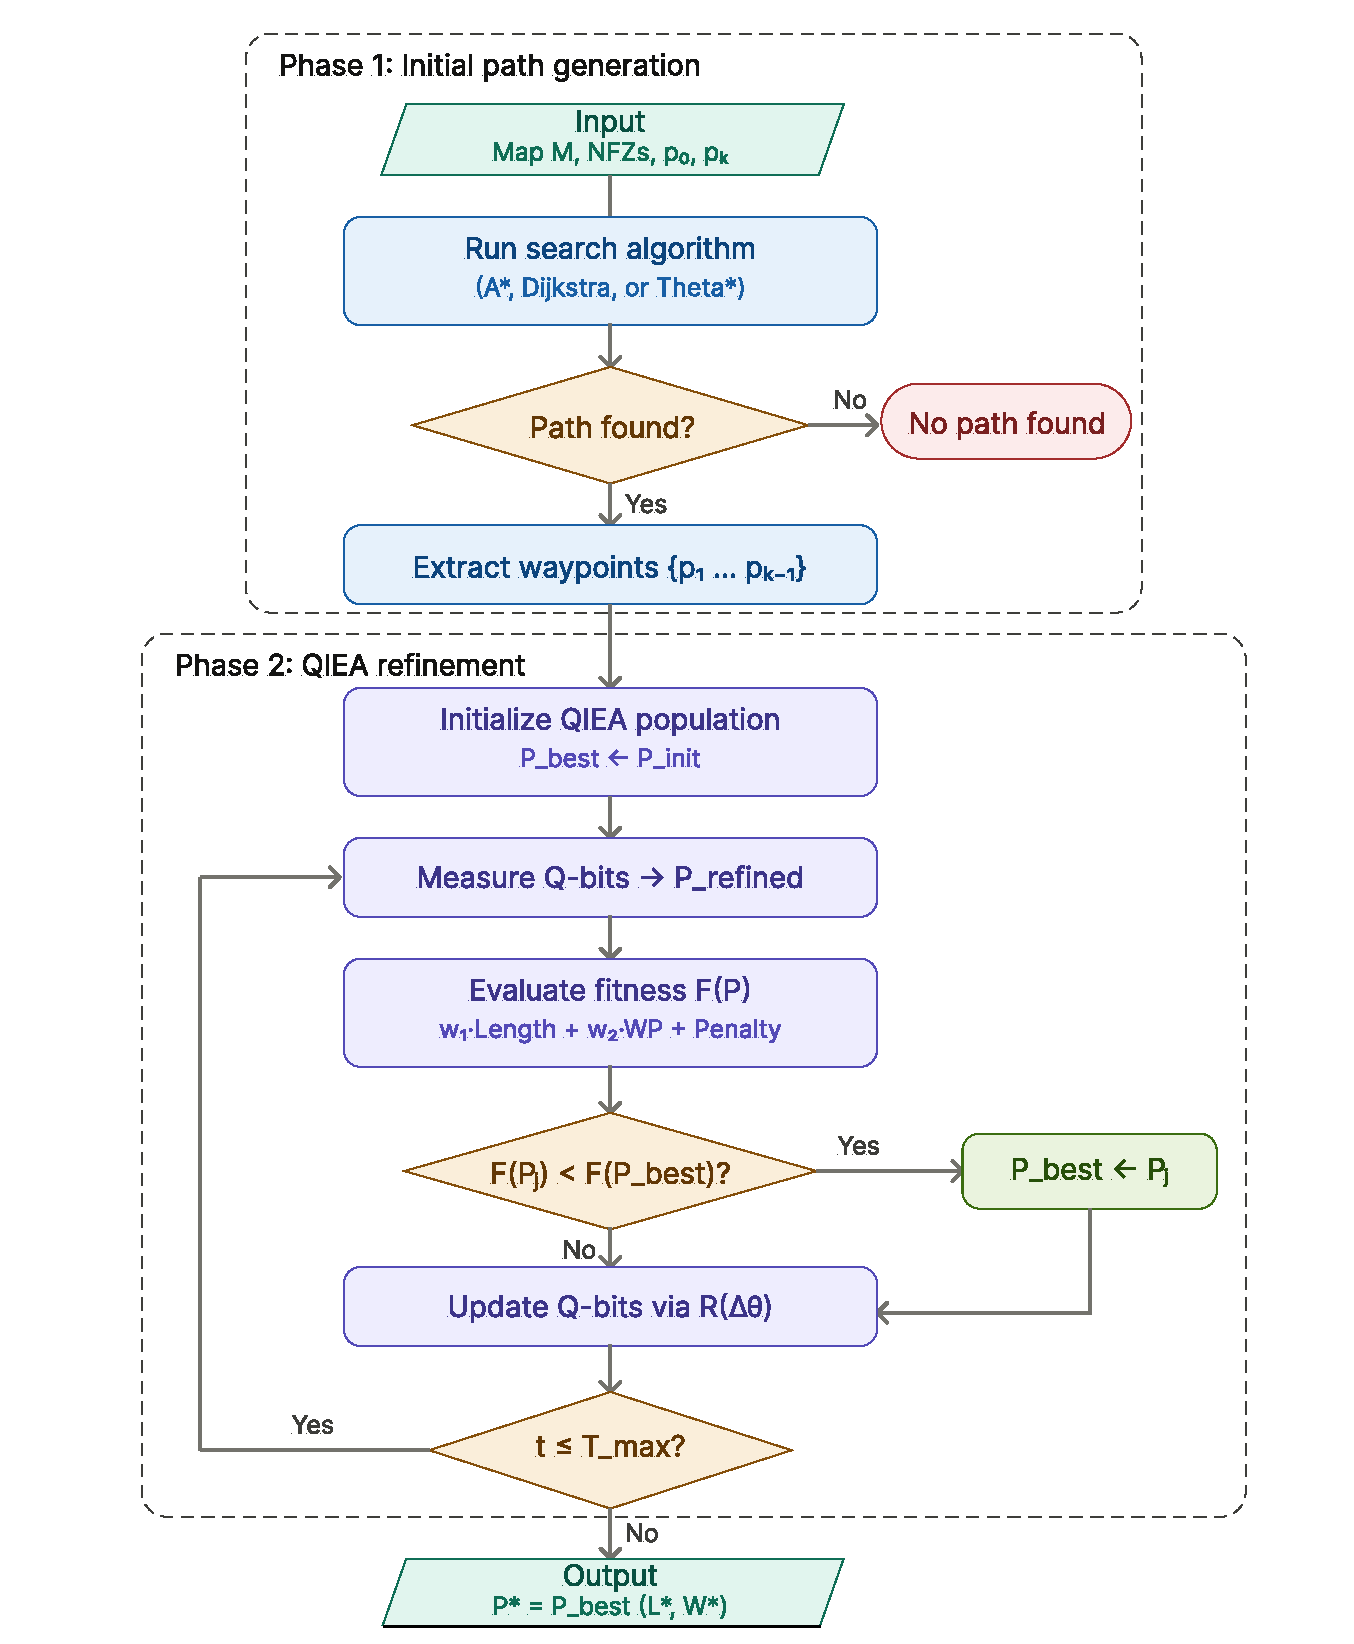
\includegraphics[width=.7\textwidth]{main-flow-v2.pdf}
    \caption{Main workflow of the proposed Hybrid Trajectory Optimization Algorithm. Phase 1 generates an initial feasible path using classical search methods (A*, Theta*, Dijkstra), which serves as the input Waypoints for Phase 2, where QIEA refines the path for optimal multi-objective cost (Length and Smoothness).}
    \label{fig:main_flow}
\end{figure}


\subsection{Phase 1: Initial Path Generation (P$_{\text{init}}$)}
The primary goal of Phase 1 is to rapidly produce a collision-free path, $P_{\text{init}}$, which guarantees feasibility within the constrained environment $\mathcal{M}$. We utilize three well-established grid-based search algorithms for this purpose: $A^{*}$, Dijkstra's, and $Theta^{*}$ \cite{ref5}. While all three guarantee finding a path if one exists, they yield different initial path qualities:
\begin{itemize}
    \item \textbf{$A^{*}$ and Dijkstra's:} These generate paths that strictly adhere to the grid structure, resulting in a high number of Waypoints ($k$ is large) and increased path length, serving as lower-quality starting solutions.
    \item \textbf{$Theta^{*}$:} This algorithm improves path quality by allowing line-of-sight connections, leading to a significantly lower number of initial Waypoints, $k_{\text{Theta}^{*}} < k_{\text{A}^{*}}$.
\end{itemize}
The generated path $P_{\text{init}} = \{p_0, p_1, \ldots, p_k\}$ serves as the fixed set of waypoints whose coordinates will be refined in the subsequent phase. Note that $p_0$ and $p_k$ (start and end points) are always fixed.


\subsection{Phase 2: Quantum-Inspired Evolutionary Refinement (QIEA)}
Phase 2 employs the QIEA to iteratively adjust the coordinates of the intermediate waypoints $\{p_1, \ldots, p_{k-1}\}$ to minimize the multi-objective cost function $F(P)$ defined in Equation \eqref{eq:total_cost}.

\subsubsection{Chromosome and Population Representation}
In QIEA, the fundamental unit is the \textbf{Q-bit}, which represents a superposition of states $|0\rangle$ and $|1\rangle$. A Q-bit is defined by a pair of complex numbers, $(\alpha, \beta)$, representing the probability amplitudes:
\begin{equation}
    |\psi\rangle = \alpha|0\rangle + \beta|1\rangle, \quad \text{where } |\alpha|^2 + |\beta|^2 = 1
    \label{eq:qbit}
\end{equation}
A \textbf{Q-bit Chromosome} is a vector of Q-bits used to encode the solution. Since we are optimizing the coordinates $(x_i, y_i)$ of the $k-1$ intermediate waypoints, we require $L$ Q-bits to encode each coordinate (if $L$ is the bit-length for the spatial dimension).

The chromosome vector $Q$ has a length of $2 \times (k-1) \times L$. The coordinates of waypoint $p_i = (x_i, y_i)$ are encoded such that the measurement of a segment of $L$ Q-bits determines the precise value of $x_i$ or $y_i$ in the continuous space $\mathcal{M}$ (ranging from 0 to $W$ or 0 to $H$) \cite{ref15}. The total Q-bit chromosome $Q$ is defined as:
\begin{equation}
    Q = [Q_{x_1}, Q_{y_1}, Q_{x_2}, Q_{y_2}, \ldots, Q_{x_{k-1}}, Q_{y_{k-1}}]
\end{equation}
where $Q_{x_i}$ and $Q_{y_i}$ are $L$-bit Q-vectors encoding the position of waypoint $p_i$.


\subsubsection{Initialization and Measurement}
The QIEA population, $Pop$, is initialized with $N$ Q-bit chromosomes. To maximize the initial diversity and search potential, all Q-bits are typically initialized to an equal superposition state: $\alpha = \beta = 1/\sqrt{2}$.

The process of generating a specific path, $P_{\text{refined}}$, from a Q-bit chromosome $Q$ is called \textbf{Measurement} (or collapse). For each Q-bit, a random number is compared against $|\alpha|^2$. If the number is less than $|\alpha|^2$, the Q-bit collapses to state $|0\rangle$; otherwise, it collapses to $|1\rangle$. This yields a classical binary string, which is then decoded to produce the real-valued coordinates of the intermediate waypoints $\{p_1, \ldots, p_{k-1}\}$. The measured Waypoints are combined with the fixed start and end points to form $P_{\text{refined}}$.


\subsubsection{Fitness Evaluation and Update Mechanism}
The fitness of the measured path $P_{\text{refined}}$ is determined by the total cost function $F(P)$ given by Equation \eqref{eq:total_cost}.

The core evolutionary mechanism in QIEA is the \textbf{Quantum Rotation Gate} ($U(\theta)$), which replaces traditional crossover and mutation operations. This gate updates the probability amplitudes $(\alpha, \beta)$ of the Q-bits in $Q$ to steer the search towards the best-known solution, $P_{\text{best}}$ (the path with the minimum fitness found so far). The rotation gate is applied as follows:
\begin{equation}
    \begin{bmatrix} \alpha_{i}^{t+1} \\ \beta_{i}^{t+1} \end{bmatrix} = R(\Delta \theta_i) \begin{bmatrix} \alpha_{i}^{t} \\ \beta_{i}^{t} \end{bmatrix} = \begin{bmatrix} \cos(\Delta \theta_i) & -\sin(\Delta \theta_i) \\ \sin(\Delta \theta_i) & \cos(\Delta \theta_i) \end{bmatrix} \begin{bmatrix} \alpha_{i}^{t} \\ \beta_{i}^{t} \end{bmatrix}
    \label{eq:rotation_gate}
\end{equation}
The magnitude and direction of the rotation angle $\Delta \theta_i$ are determined based on the comparison between the current measured solution and the corresponding Q-bits in $P_{\text{best}}$. The update rule ensures that Q-bits with better fitness values are retained and reinforced in the population, facilitating faster convergence toward the optimal region of the continuous search space \cite{ref16}.

\subsubsection{Feasibility Check and Constraint Handling}
Since the QIEA operates in continuous space, the refined path $P_{\text{refined}}$ may violate the collision constraint by intersecting one or more NFZs. The constraint handling is performed implicitly via the penalty term $C_{\text{penalty}}$ (Equation \eqref{eq:cost_penalty}).

For every measured path $P_{\text{refined}}$, a geometry check is performed to test if any segment connecting $p_{i-1}$ and $p_i$ intersects $S_{\text{obs}}$. If a collision is detected, the path is immediately assigned the maximum penalty cost $M$. This mechanism strongly penalizes infeasible solutions during the fitness evaluation, guiding the QIEA to explore only the collision-free space near the initial feasible path $P_{\text{init}}$.

\begin{center}
\begin{minipage}{0.9\textwidth}
\centering
\small\refstepcounter{algorithm}\label{alg:hybrid_qiea}\textbf{Algorithm \thealgorithm.} Hybrid Path Optimization Algorithm (Search + QIEA)
\par\medskip\hrule
\begin{enumerate}
\item \textbf{Input:} Map $\mathcal{M}$, Start $p_{\text{start}}$, End $p_{\text{end}}$, QIEA parameters ($N$, $T_{max}$).
\item \textbf{Output:} Optimal Trajectory $P^{*}$.
\item \textbf{Phase 1: Initial Path Generation}
\item Select Search Algorithm (A*, Theta*, or Dijkstra).
\item $P_{\text{init}} \gets \text{Search}(p_{\text{start}}, p_{\text{end}}, \mathcal{M})$
\item If $P_{\text{init}}$ is null, return ``No path found.''
\item Identify intermediate Waypoints $\{p_1, \ldots, p_{k-1}\}$ from $P_{\text{init}}$.
\item \textbf{Phase 2: QIEA Refinement}
\item Initialize Population $Pop$ of $N$ Q-bit Chromosomes based on $k-1$ Waypoints.
\item $P_{\text{best}} \gets P_{\text{init}}$
\item For $t = 1$ to $T_{max}$:
\begin{enumerate}
\item \textbf{Measurement:} $P_{\text{pop\_refined}} \gets \text{Measure}(Pop)$
\item \textbf{Fitness Evaluation and Selection:} For each $P_{j} \in P_{\text{pop\_refined}}$, calculate $F(P_{j})$ using Equation~\eqref{eq:total_cost}; if $F(P_{j}) < F(P_{\text{best}})$ then $P_{\text{best}} \gets P_{j}$.
\item \textbf{Update:} $Pop \gets \text{UpdateUsingRotationGates}(Pop, P_{\text{best}})$
\end{enumerate}
\item Return $P^* = P_{\text{best}}$
\end{enumerate}
\par\smallskip\hrule
\end{minipage}
\end{center}

\noindent The Hybrid Algorithm operates sequentially, as summarized in Algorithm 1. \textbf{Phase 1} (Steps 3--7) rapidly generates an initial collision-free path, $P_{\text{init}}$, using a selected classical search algorithm ($A^*$, Dijkstra, or $Theta^*$). This initial path guarantees feasibility and provides the fixed set of intermediate waypoints $\{p_1, \ldots, p_{k-1}\}$. In \textbf{Phase 2} (Steps 8--12), these intermediate waypoints define the structure of the QIEA's initial population ($Pop$). The QIEA then iteratively refines the coordinates in the continuous search space by measuring Q-bit chromosomes ($P_{\text{pop\_refined}}$), evaluating fitness against the multi-objective cost $F(P)$, and updating the population using quantum rotation gates guided by the current best solution ($P_{\text{best}}$). The process ensures that optimization starts from a feasible point and maintains feasibility through continuous penalty checks against NFZs.


%-------------------------------------------------------------------------

\section{EXPERIMENTS AND RESULTS}
\label{sec:experiments}

This section presents the simulation setup, evaluation metrics, and a detailed analysis of the performance of the proposed hybrid optimization algorithms against their classical baseline counterparts.


\subsection{Simulation Environment and Setup}

Our experimental environment is a 2D discrete grid map $\mathcal{M}$ of size $50 \times 50$ units, representative of a localized aerial service area. Obstacles are modeled as \textbf{Non-Fly Zones (NFZs)}, which are defined by multiple circular regions of varying radii, simulating diverse restricted areas and risk levels. The starting point (\textit{green circle}) and the goal point (\textit{blue star}) were fixed for all comparative runs on this specific map instance, ensuring a consistent benchmark. The NFZs are visually depicted as pink-red shaded circles.

We compare the performance of three baseline search algorithms ($A^{*}$, Dijkstra's, and $Theta^{*}$) with their hybrid counterparts ($A^{*}$+QIEA, Dijkstra+QIEA, and $Theta^{*}$+QIEA).

The parameters for the QIEA refinement phase (Phase 2) were set empirically to ensure a balance between convergence speed and solution quality. Key parameters include: a \textbf{Population Size ($N$)} of 50 Q-bit chromosomes, a \textbf{Maximum Generations ($T_{max}$)} of 200, and an \textbf{Adaptive Rotation Angle ($\Delta \theta$)} with an initial learning rate calibrated around $\pm 0.05\pi$. For the multi-objective cost function $F(P)$, weights were set at $w_1=0.6$ (for Length) and $w_2=0.4$ (for Waypoints), slightly prioritizing path length over smoothness. The \textbf{Penalty ($M$)} for collision was set to $10^6$ to ensure immediate rejection of infeasible paths.

All experiments were conducted on grid-based environments of size $50 \times 50$ with circular NFZs. To assess robustness and generalizability, three different map instances with varying NFZ configurations were evaluated, maintaining the same start and goal locations for fair comparison across different planners. To analyze the influence of objective weighting, three representative weight configurations were considered: \textit{Waypoint-prioritized} (emphasizing trajectory smoothness), \textit{Length-prioritized} (emphasizing shortest path length), and \textit{Balanced} (providing a trade-off). All other algorithmic parameters remained unchanged across experiments.


\subsection{Performance Metrics}

The algorithms are evaluated based on three primary metrics:

\begin{itemize}
    \item \textbf{Path Length:} The total Euclidean distance traveled, $C_{\text{length}}(P)$. Lower values indicate better overall length optimality and energy efficiency.
    \item \textbf{Waypoints:} The number of segments, $k$, in the trajectory. This serves as a direct measure of path smoothness, where fewer Waypoints imply reduced maneuvering effort for the UAV.
    \item \textbf{Computation Time (s):} The total time taken by the algorithm (Search + Refinement) to find the solution.
\end{itemize}



\subsection{Results Analysis}

To visually compare the effectiveness of the QIEA refinement, Figure~\ref{fig:visual_comparison} presents the trajectories generated by all six algorithms on the same $50 \times 50$ test map. The starting point is marked by a green circle, the goal by a blue star, and NFZs are shown in pink-red. Table~\ref{tab:comparison_results} presents a summary of the measured performance metrics for all six algorithms on the $50 \times 50$ test map instance.


% Visual result by images

\begin{figure}[htbp]
\centering
\begin{minipage}{\textwidth}
    \centering
    % Row 1: Baseline algorithms
    \begin{subfigure}[t]{0.32\textwidth}
        \centering
        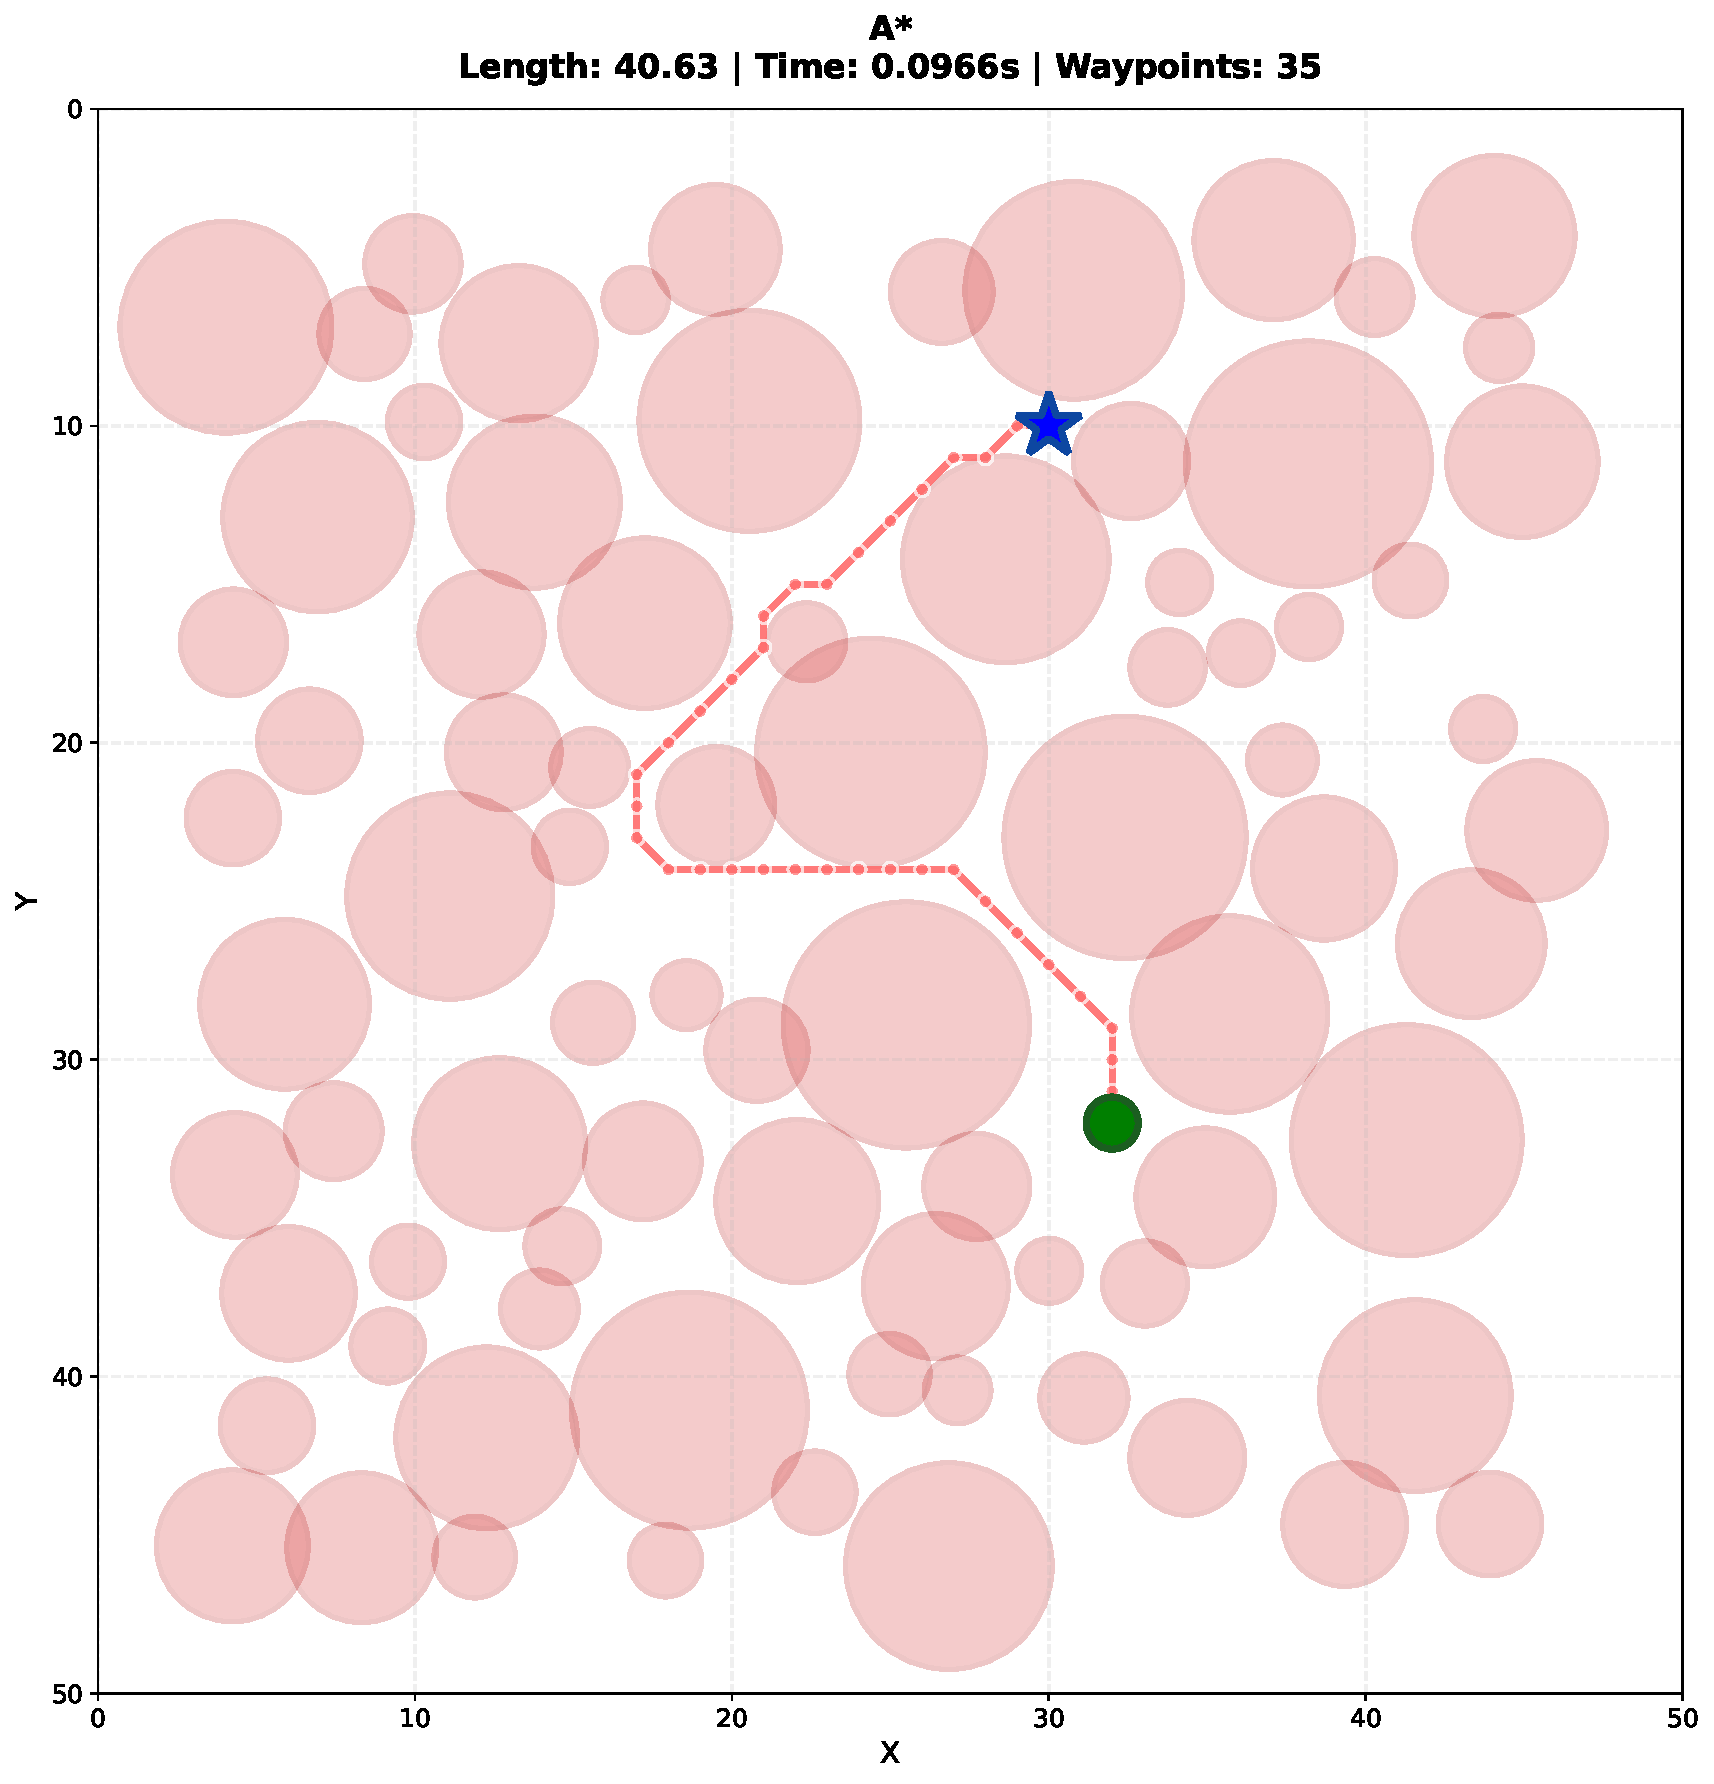
\includegraphics[width=\linewidth]{m1_50x50_Astar.pdf}
        \caption{\small Baseline A*: L=40.63, W=35. Time=0.0966s.}
        \label{fig:Astar_baseline}
    \end{subfigure}\hfill%
    \begin{subfigure}[t]{0.32\textwidth}
        \centering
        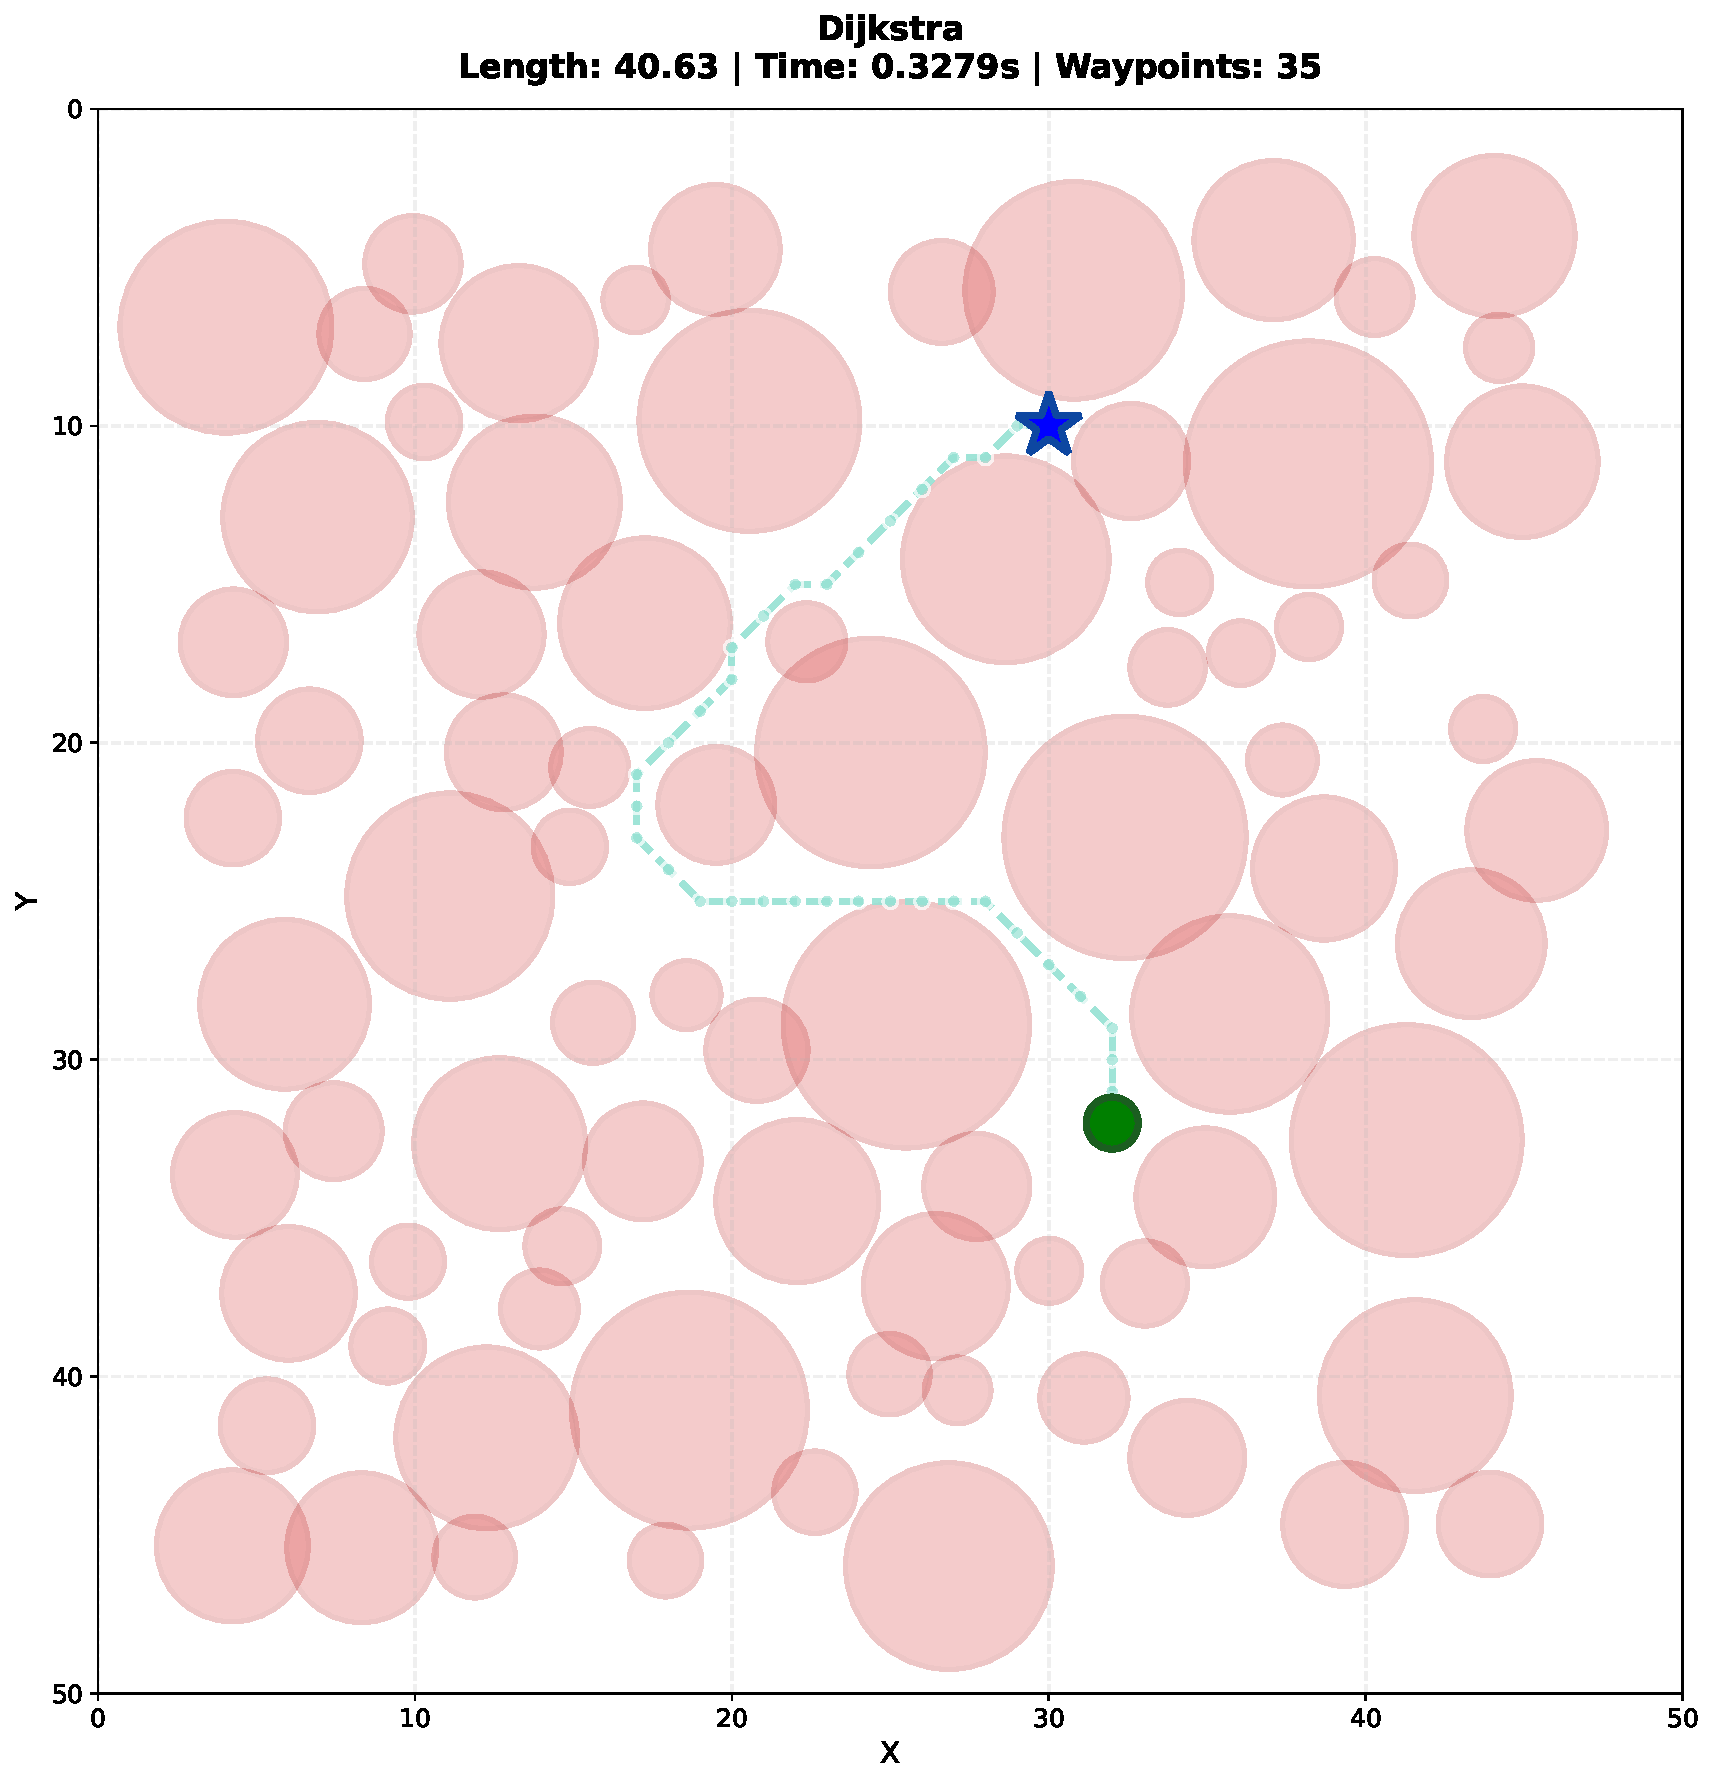
\includegraphics[width=\linewidth]{m1_50x50_Dijkstra.pdf}
        \caption{\small Baseline Dijkstra: L=40.63, W=35. Time=0.3279s.}
        \label{fig:Dijkstra_baseline}
    \end{subfigure}\hfill%
    \begin{subfigure}[t]{0.32\textwidth}
        \centering
        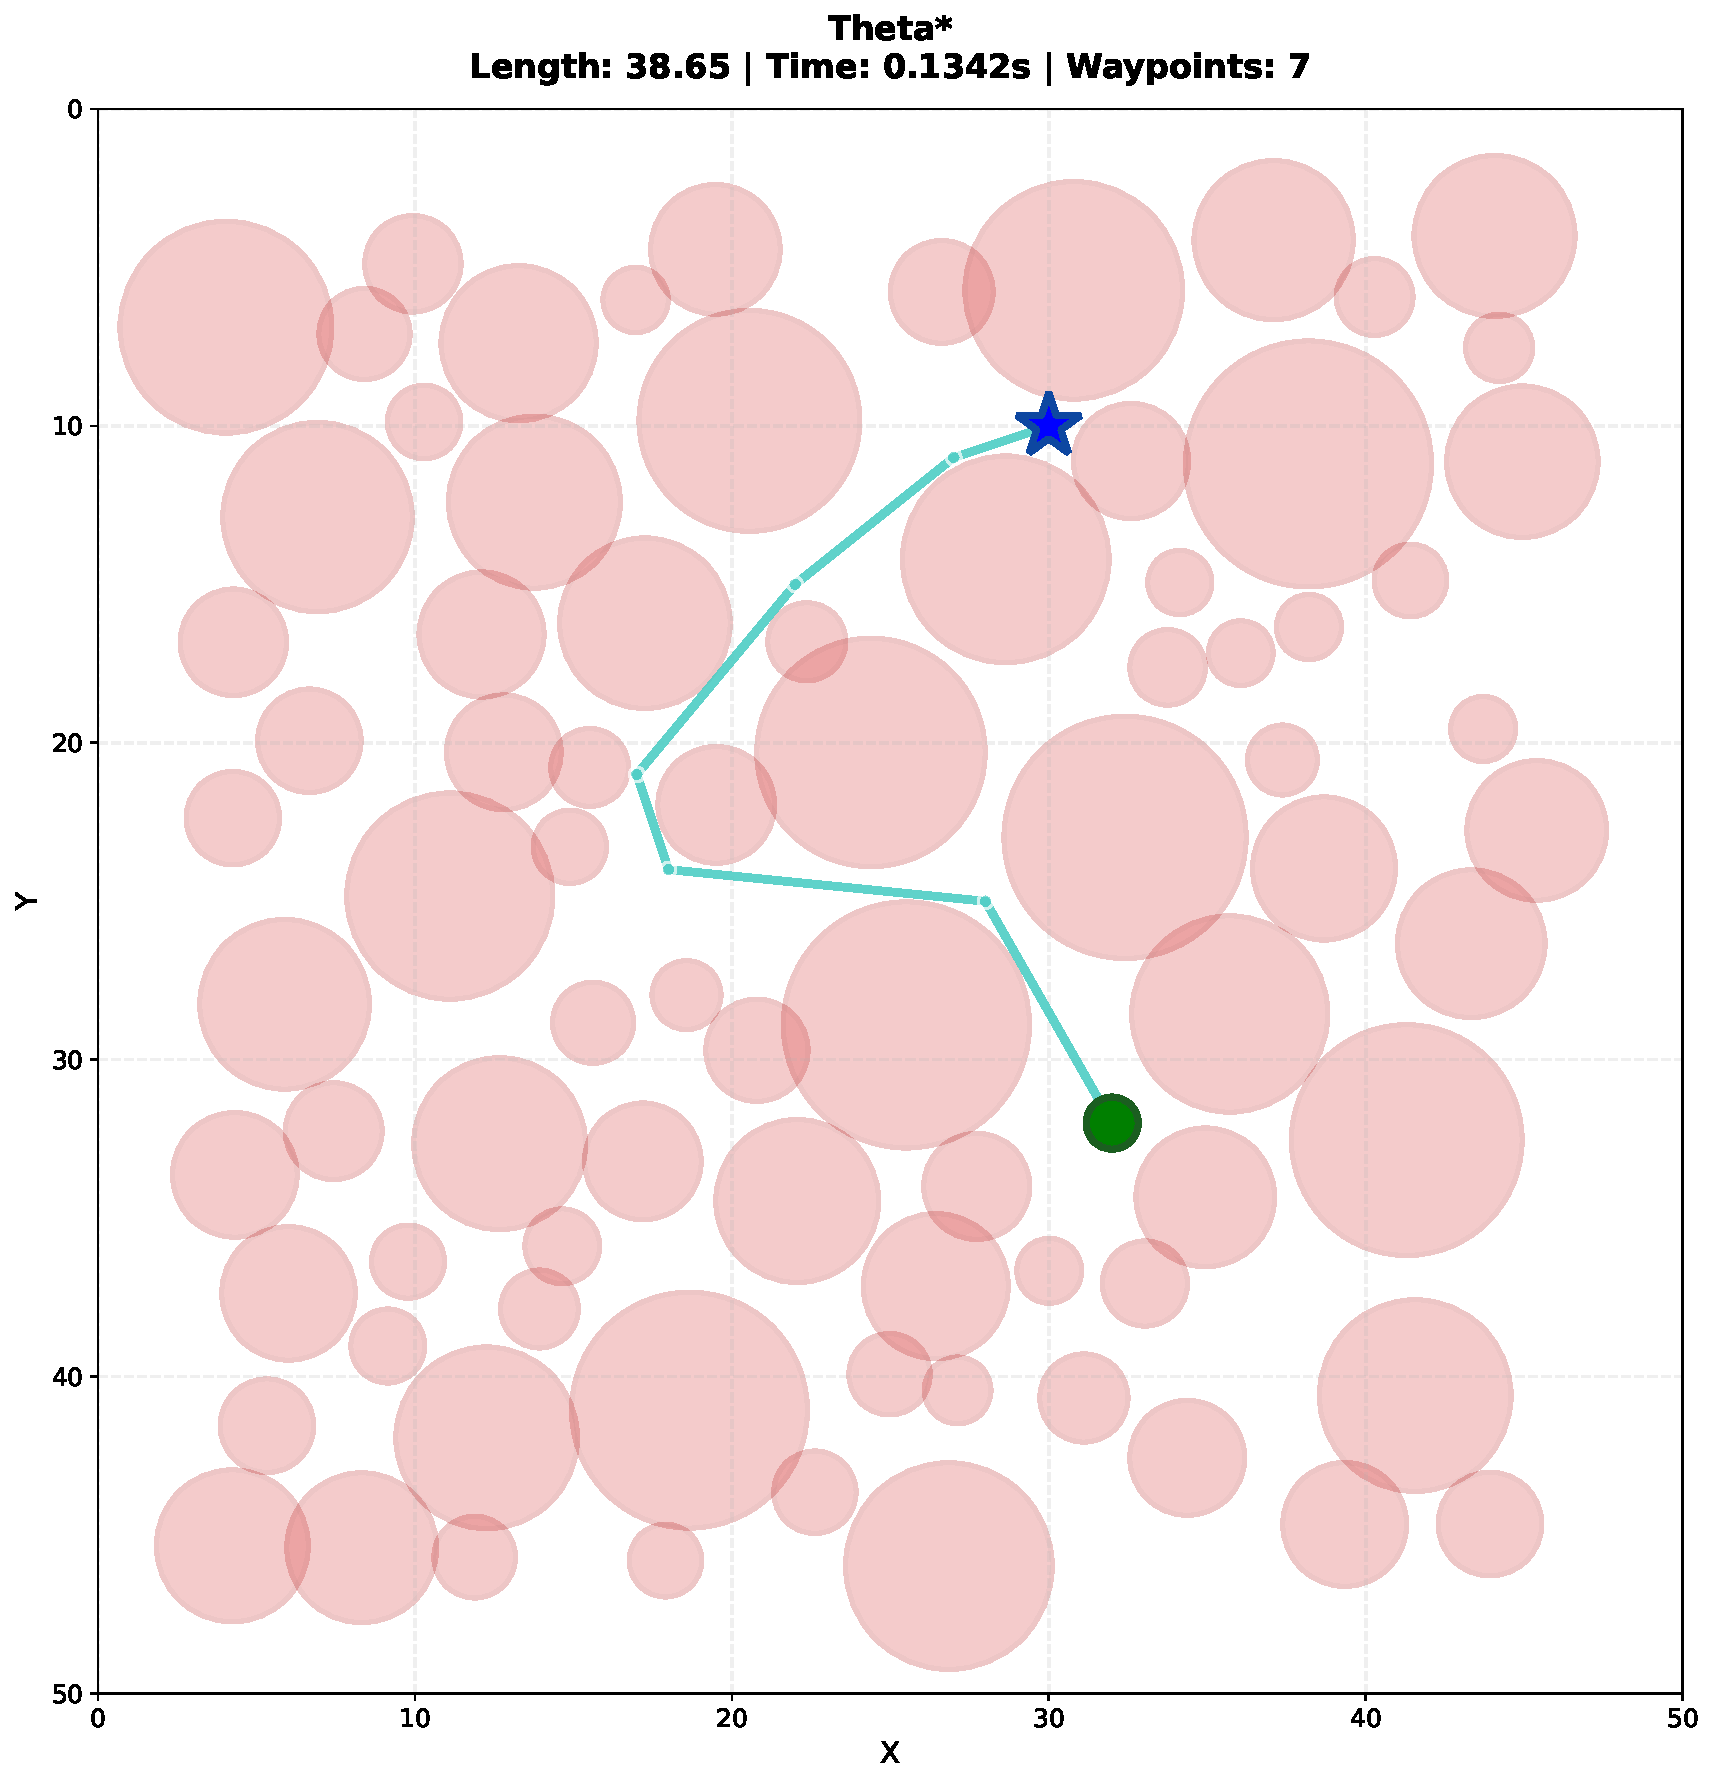
\includegraphics[width=\linewidth]{m1_50x50_Thetastar.pdf}
        \caption{\small Baseline Theta*: L=38.65, W=7. Time=0.1342s.}
        \label{fig:Thetastar_baseline}
    \end{subfigure}

    \vspace{0.4cm}

    % Row 2: Hybrid algorithms (QIEA refined)
    \begin{subfigure}[t]{0.32\textwidth}
        \centering
        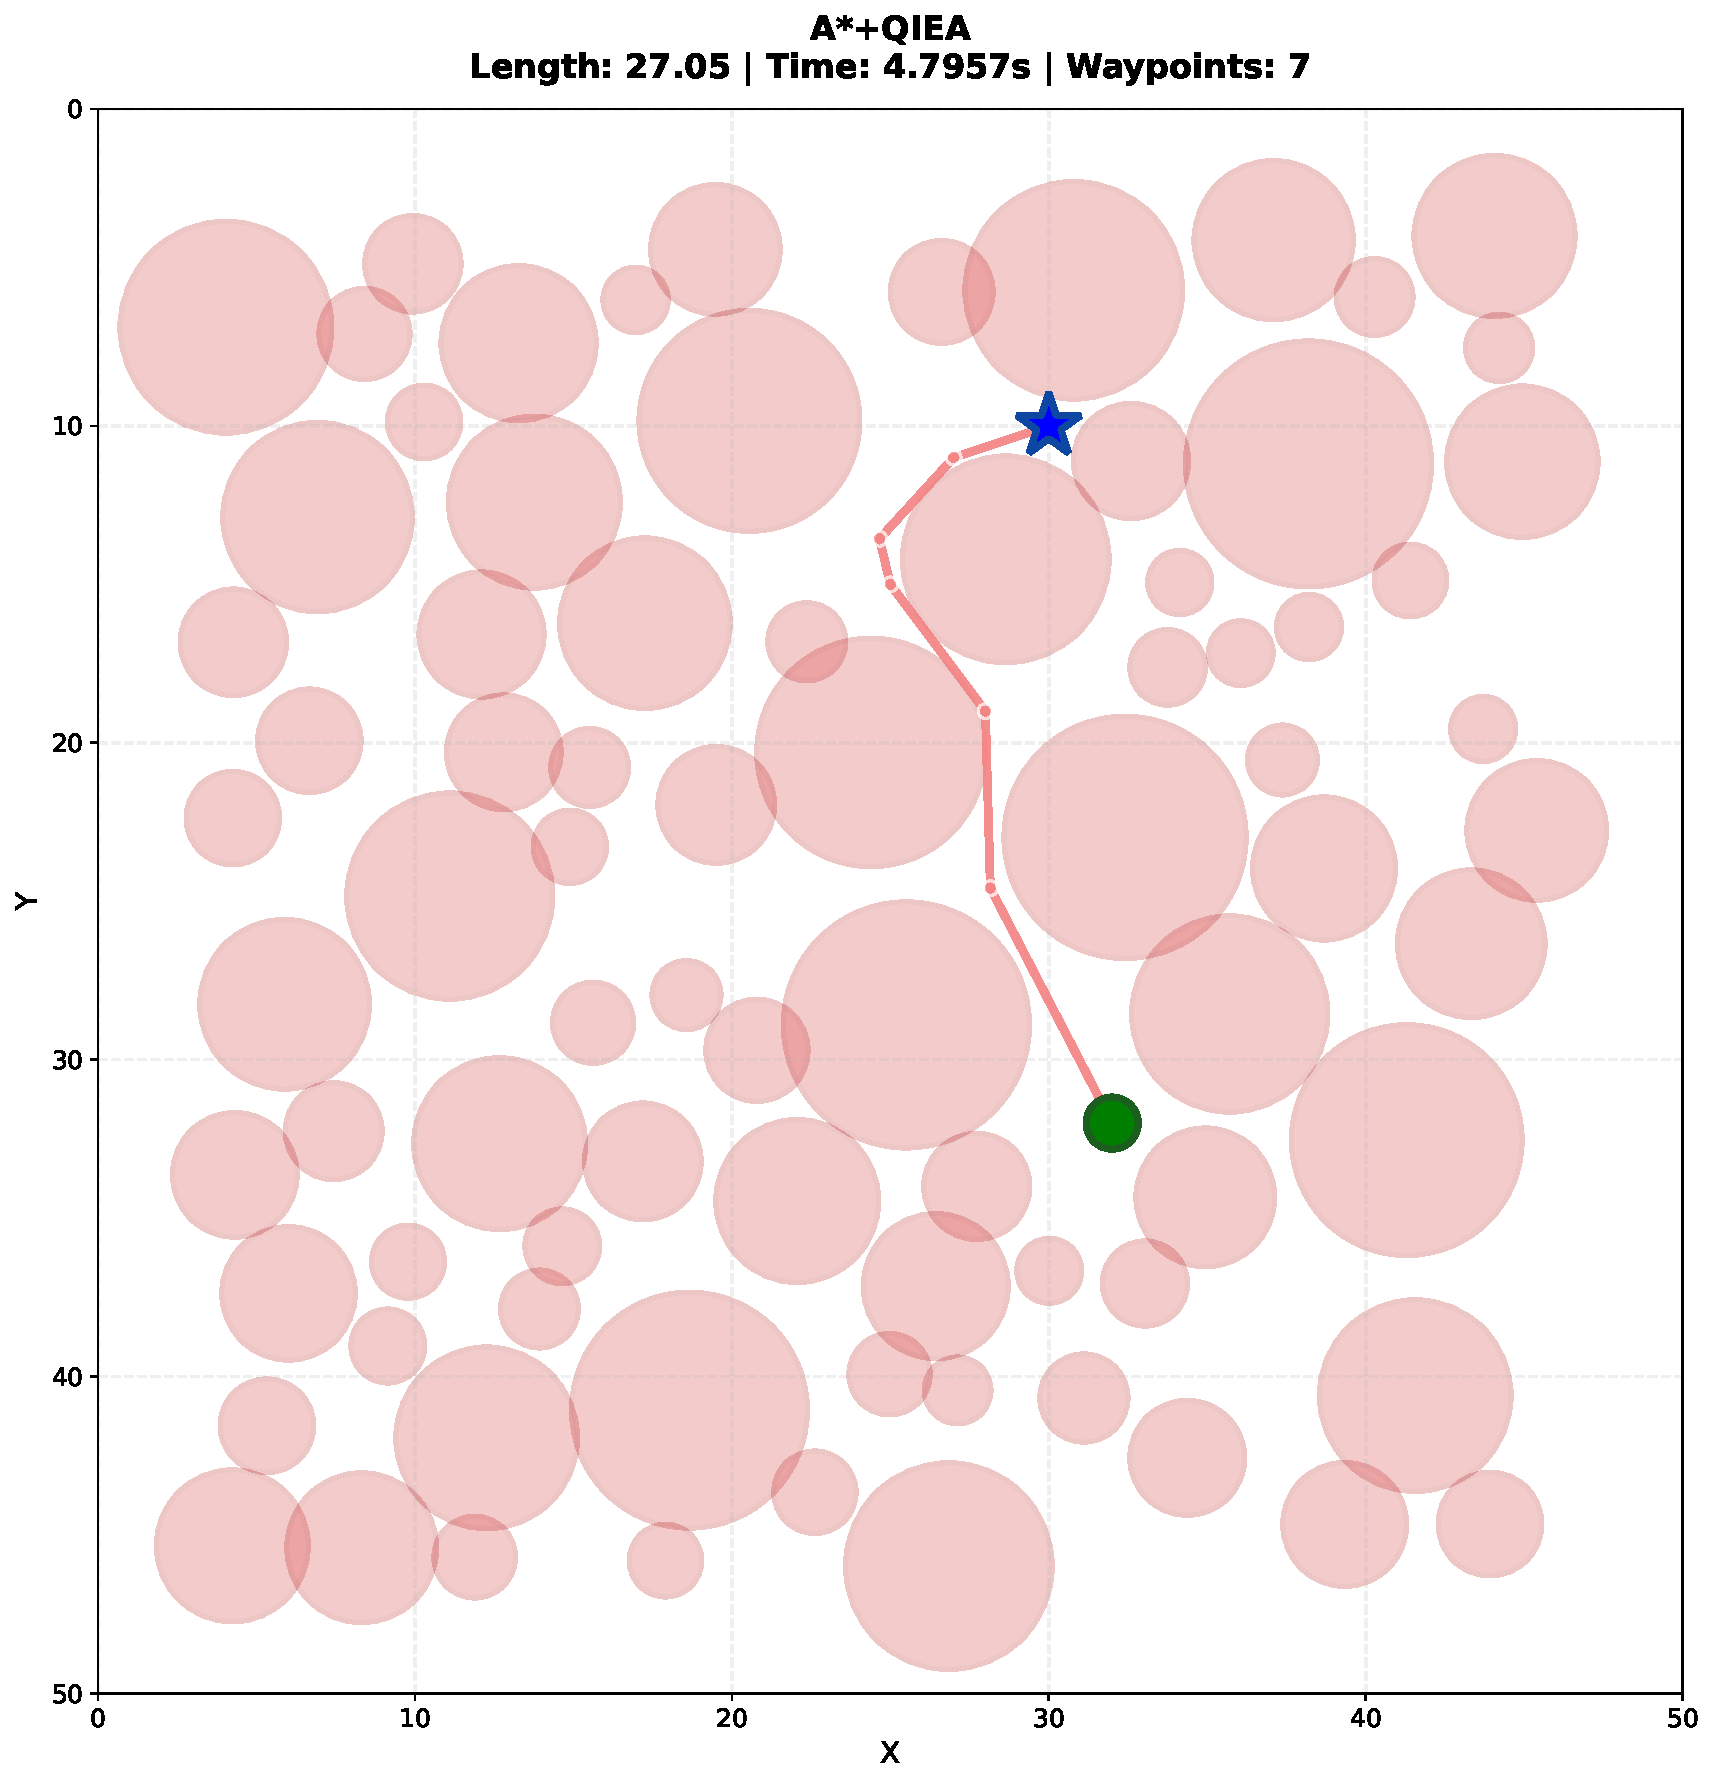
\includegraphics[width=\linewidth]{m1_50x50_AstarplusQIEA.pdf}
        \caption{\small Hybrid A*+QIEA: \textbf{L=27.05}, W=7. Time=4.7957s.}
        \label{fig:Astar_hybrid}
    \end{subfigure}\hfill%
    \begin{subfigure}[t]{0.32\textwidth}
        \centering
        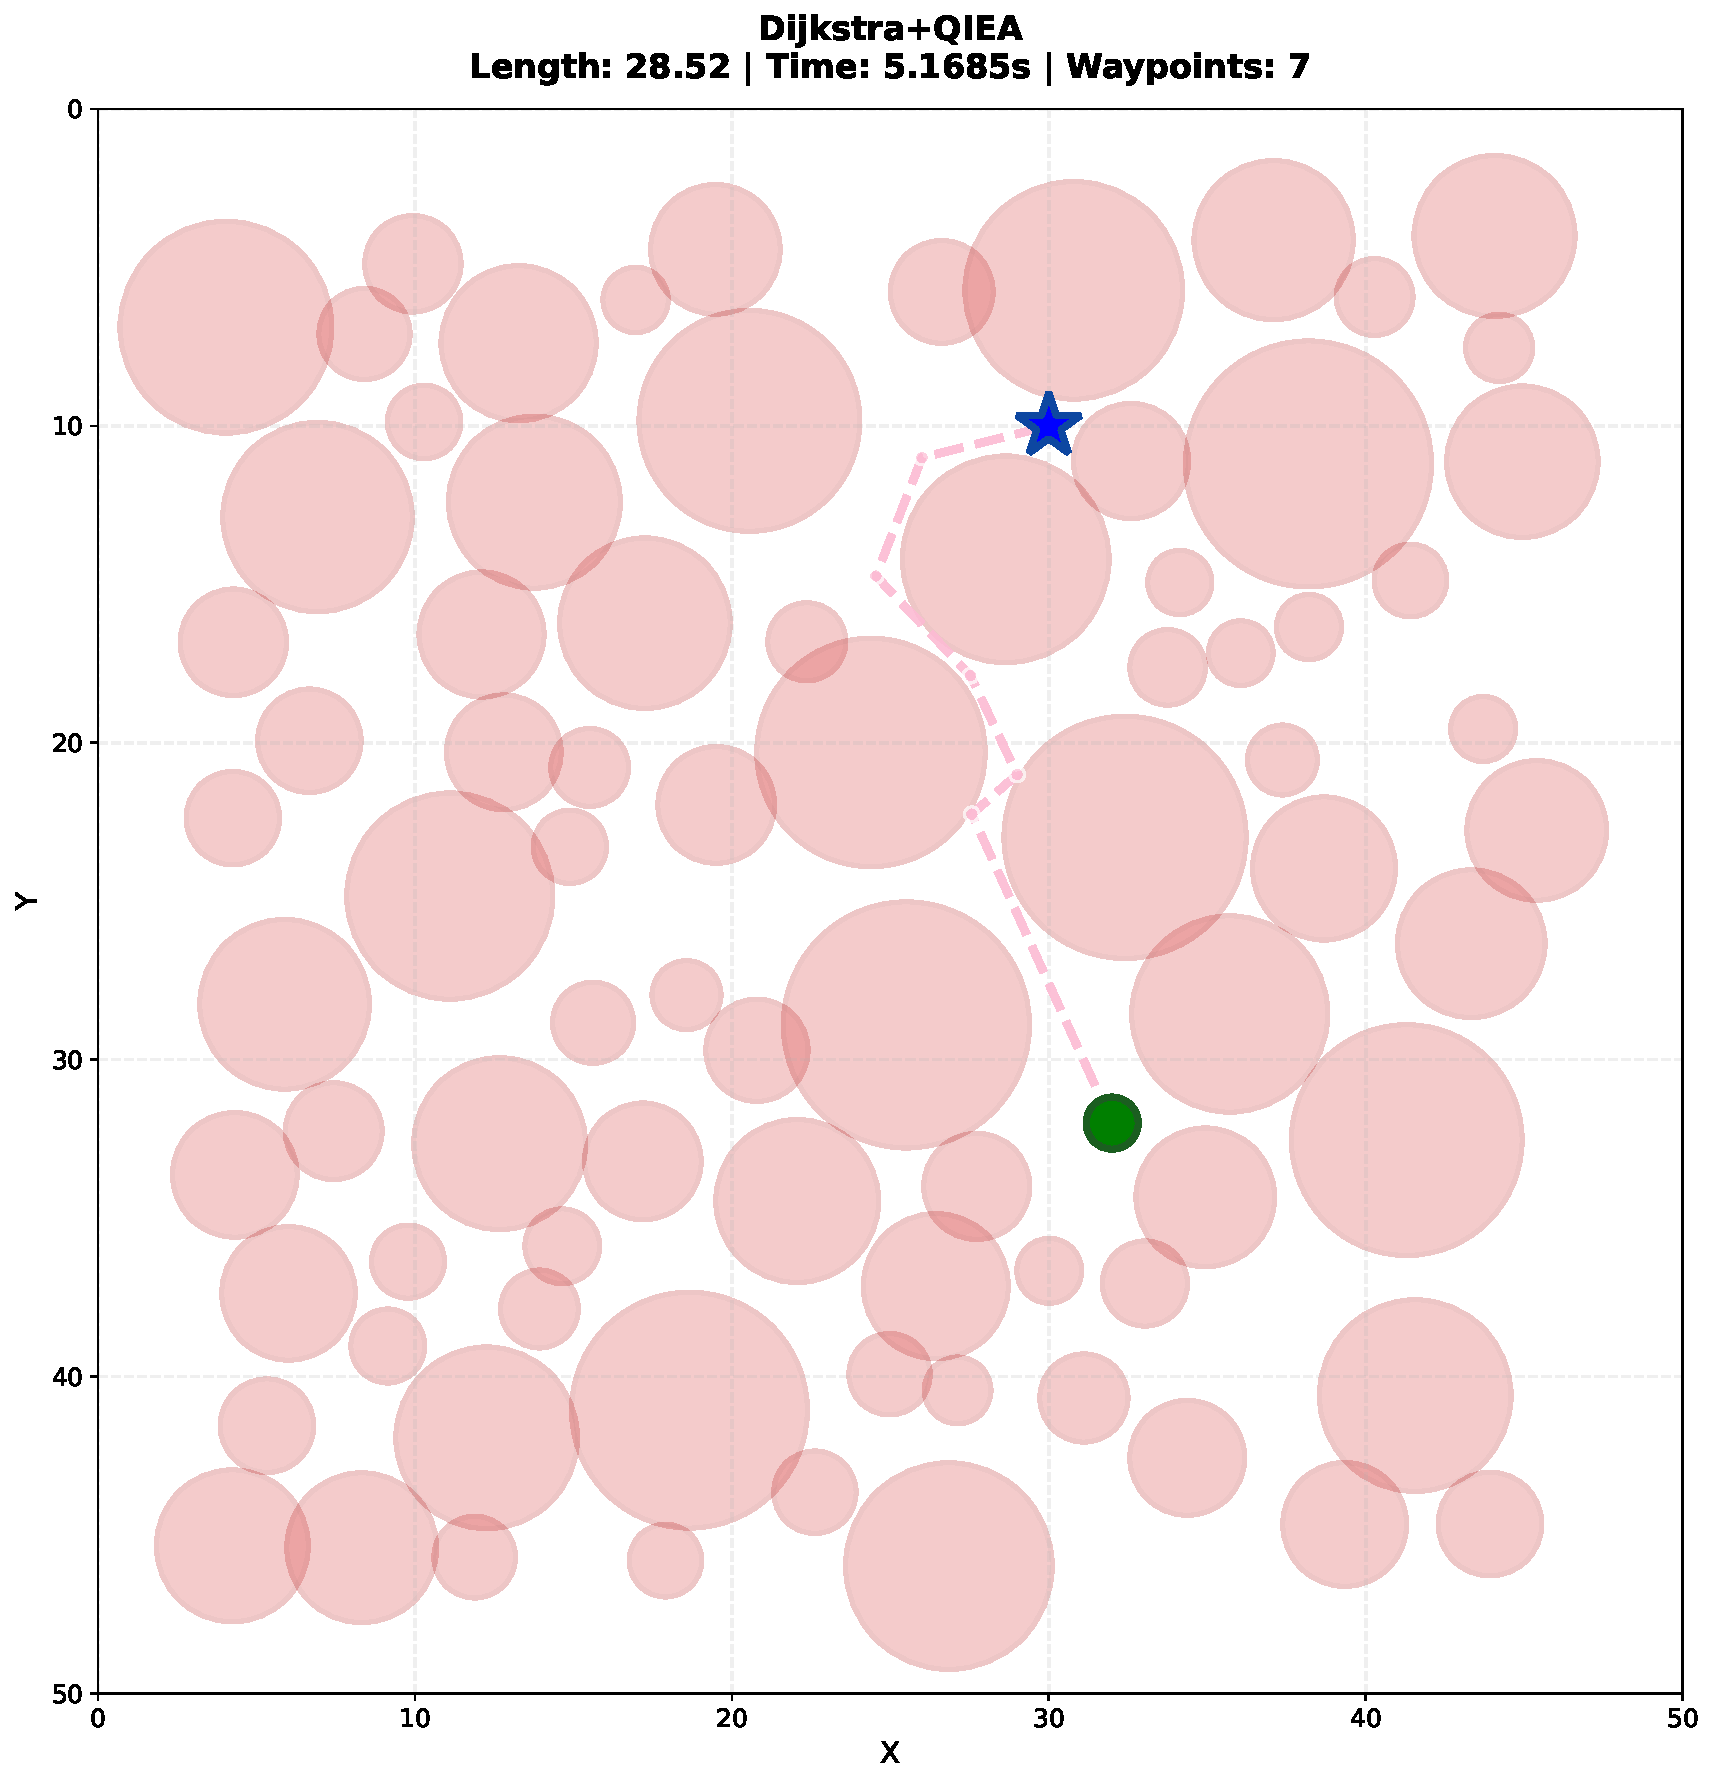
\includegraphics[width=\linewidth]{m1_50x50_DijkstraplusQIEA.pdf}
        \caption{\small Hybrid Dijkstra+QIEA: L=28.52, W=7. Time=5.1685s.}
        \label{fig:Dijkstra_hybrid}
    \end{subfigure}\hfill%
    \begin{subfigure}[t]{0.32\textwidth}
        \centering
        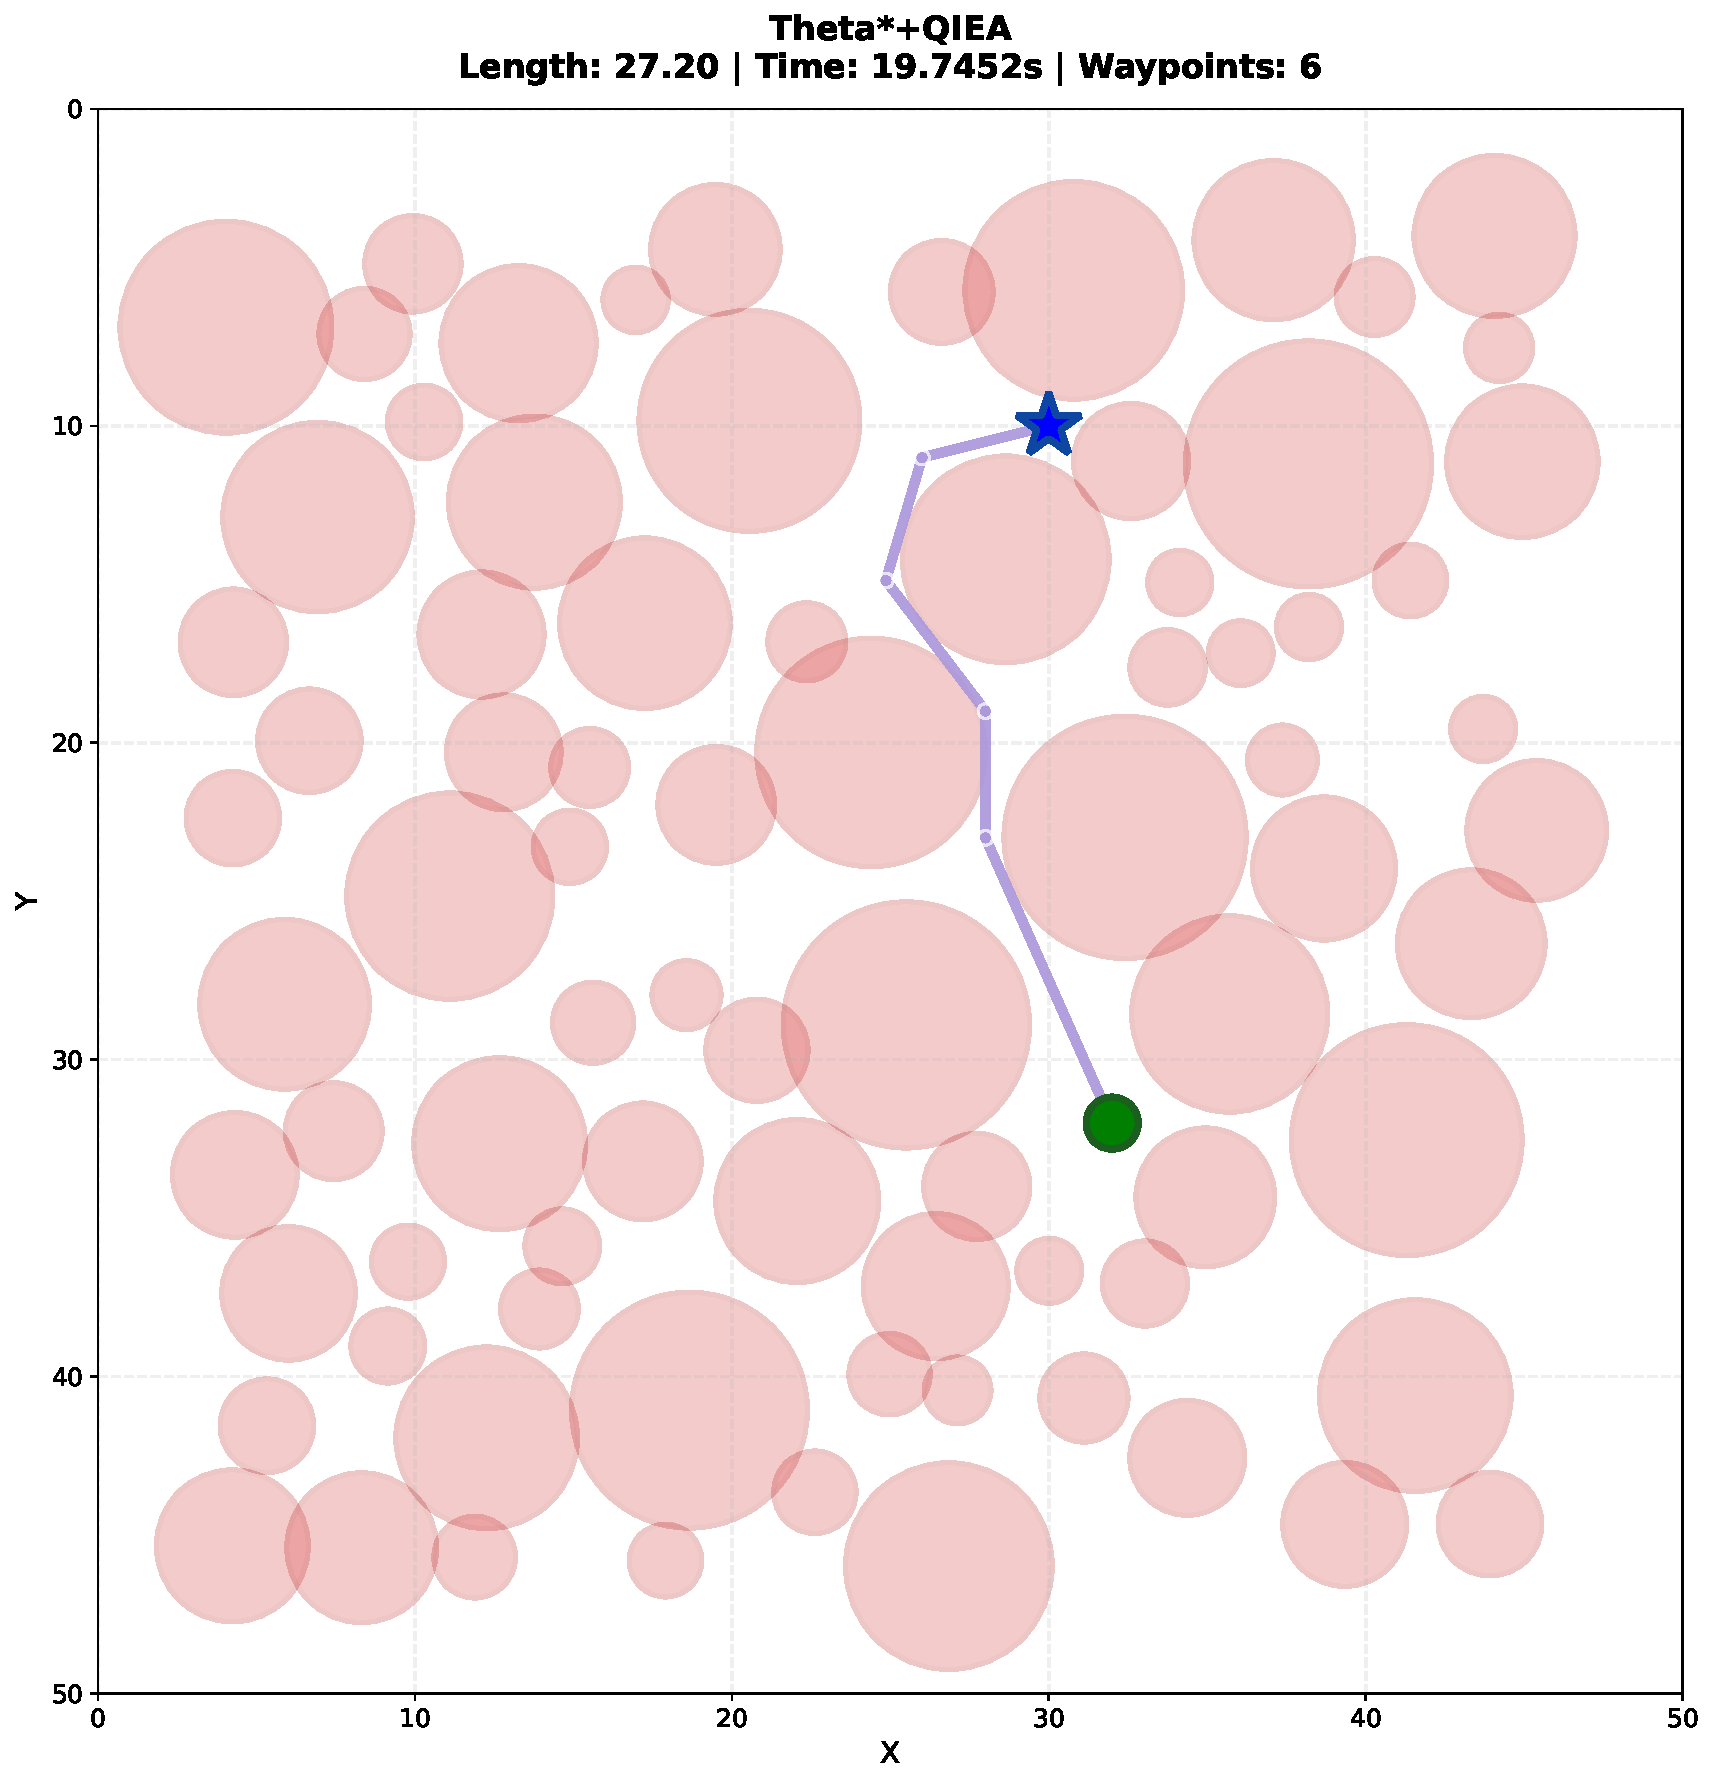
\includegraphics[width=\linewidth]{m1_50x50_ThetastarplusQIEA.pdf}
        \caption{\small Hybrid Theta*+QIEA: L=27.20, \textbf{W=6}. Time=19.7452s.}
        \label{fig:Thetastar_hybrid}
    \end{subfigure}
\end{minipage}
\caption{\small Visual comparison of the trajectory results. The top row shows the discrete paths from baseline search methods; the bottom row shows the effect of QIEA refinement, yielding shorter and smoother continuous-space trajectories around the circular NFZs.}
\label{fig:visual_comparison}
\end{figure}


\begin{table}[t]
\centering
\caption{\small Comparison of Baseline and Hybrid Path Planning Algorithms on 50$\times$50 Map.}
\label{tab:comparison_results}
\begin{tabular}{l l c c c}
\hline
\textbf{Algorithm} & \textbf{Type} & \textbf{L} & \textbf{W} & \textbf{Time (s)} \\
\hline
A* & Baseline & 40.63 & 35 & 0.0966 \\
Dijkstra & Baseline & 40.63 & 35 & 0.3279 \\
Theta* & Baseline & 38.65 & 7 & 0.1342 \\
A*+QIEA & Hybrid & \textbf{27.05} & 7 & 4.7957 \\
Dijkstra+QIEA & Hybrid & 28.52 & 7 & 5.1685 \\
Theta*+QIEA & Hybrid & 27.20 & \textbf{6} & 19.7452 \\
\hline
\end{tabular}
\end{table}





% ================================================
\subsubsection{Sensitivity weights and experimental results}

Sensitivity weights allow for adjustment of the trade-off between path length and number of waypoints. Table~\ref{tab:weights} describes the three configurations used in the experiments. Table~\ref{tab:waypoints} reports the results on three maps ($50\times50$) for the \emph{prioritize waypoints} configuration.

\begin{table}[htbp]
\centering
\small
\caption{\small Sensitivity weight configurations for Length and Waypoints.}
\label{tab:weights}
\begin{tabular}{l p{6cm}}
\hline
\textbf{Configuration} & \textbf{Description (weights)} \\
\hline
Prioritize waypoints & Higher weight on minimizing waypoints; lower weight on length. \\
Prioritize length & Higher weight on minimizing path length; lower weight on waypoints. \\
Balanced & Equal or comparable weights for length and waypoints. \\
\hline
\end{tabular}
\end{table}


\begin{table}[htbp]
\centering
\small
\renewcommand{\arraystretch}{1.2}
\caption{\small Results with config \emph{prioritize waypoints} on three maps. L = Length, T = Time (s), W = Waypoints.}
\label{tab:waypoints}
\begin{tabular}{l c c c}
\hline
\textbf{Method} & \textbf{Map 1} & \textbf{Map 2} & \textbf{Map 3} \\
& \textit{m1\_50x50\_v1} & \textit{m1\_50x50\_v2} & \textit{m1\_50x50\_v3} \\
& L / T (s) / W & L / T (s) / W & L / T (s) / W \\
\hline
A* & 40.63 / 0.095 / 35 & 73.53 / 0.352 / 65 & 50.63 / 0.137 / 45 \\
Theta* & 38.65 / 0.139 / 7 & 71.61 / 0.480 / 15 & 47.68 / 0.128 / 5 \\
Dijkstra & 40.63 / 0.329 / 35 & 73.53 / 0.584 / 65 & 50.63 / 0.534 / 45 \\
A*+QIEA & 27.90 / 4.79 / 8 & 73.53 / 3.83 / 65 & 48.14 / 3.10 / 4 \\
Theta*+QIEA & 28.02 / 19.59 / 6 & 71.61 / 13.17 / 15 & 47.92 / 9.93 / 4 \\
Dijkstra+QIEA & 27.87 / 4.84 / 6 & 73.53 / 3.98 / 65 & 47.96 / 3.19 / 4 \\
\hline
\end{tabular}
\end{table}


Table~\ref{tab:waypoints} presents the results of the \emph{prioritize waypoints} configuration across the three map instances. On Map~1, the hybrid methods achieve substantial improvements: A*+QIEA reduces path length from 40.63 to 27.90 units while cutting waypoints from 35 to 8; Dijkstra+QIEA attains the lowest waypoint count (W=6) with length 27.87; and Theta*+QIEA maintains the smoothest trajectory (W=6) with length 28.02. On Map~3, all hybrids yield significantly smoother paths: A*+QIEA, Dijkstra+QIEA, and Theta*+QIEA reduce waypoints to 4, compared to 45 for baseline A* and Dijkstra. On Map~2, the hybrid methods preserve the baseline solution quality: A*+QIEA and Dijkstra+QIEA maintain L=73.53 and W=65, identical to their respective baselines, while Theta*+QIEA retains L=71.61 and W=15. This demonstrates that when the initial path is already near-optimal or tightly constrained by the obstacle geometry, QIEA does not degrade the solution-it preserves feasibility and path metrics. Thus, the hybrid framework is robust: QIEA either improves the trajectory when refinement is possible (as on Maps~1 and~3) or maintains the quality of the initial path when further optimization is limited by the environment.


%================================================

\subsubsection{Computational Trade-off}

The significant reduction in path length and complexity achieved by the hybrid methods comes at the expense of increased computation time, as the QIEA refinement phase is iterative. The baseline search algorithms execute in milliseconds (e.g., A* at 0.0971s). The hybrid methods, which incorporate 200 generations of QIEA, typically require several seconds (around 4.5s for A*+QIEA and Dijkstra+QIEA).

The trade-off is summarized as follows: for an extra 4 to 5 seconds of computation, the system gains a minimum of 30\% reduction in flight distance and a significant decrease in Waypoints. For \textbf{off-line path planning}, where the trajectory is calculated before the mission begins, this trade-off is highly advantageous and operationally sound, as the accrued benefits in energy conservation and reduced mechanical wear far outweigh the minor pre-mission computational delay.

However, it is notable that \texttt{Theta*+QIEA} took significantly longer (19.6162 s) in Map 1. This extended duration is likely attributable to the characteristics of \texttt{Theta*}'s initial path (7 Waypoints), which resulted in Waypoints being positioned closer to the NFZ boundaries or in more geometrically constrained locations. These tight initial constraints require more intricate maneuvering by the QIEA, demanding more rotation gate updates and generations to satisfy the non-collision constraint $C_{penalty}$ while successfully optimizing length and smoothness.
    
\subsubsection{Sensitivity Analysis of Objective Weights}
To investigate the sensitivity of the proposed hybrid framework to the choice of objective weights, experiments are conducted using three different weight configurations corresponding to prioritizing path length, prioritizing waypoint reduction, and a balanced trade-off.

Table~\ref{tab:comparison_results} summarizes representative results across different map instances. When the weight associated with waypoint count is increased, the optimized trajectories exhibit significantly fewer waypoints, resulting in smoother paths. Conversely, emphasizing path length leads to shorter trajectories at the cost of increased waypoint complexity. The balanced configuration achieves a compromise between these two objectives.

Importantly, across all tested maps and weight configurations, the proposed hybrid approaches never degrade the quality of the initial feasible paths generated by classical search algorithms. In cases where the initial trajectory is already near-optimal or strongly constrained by obstacle geometry, the QIEA-based refinement preserves the solution quality while maintaining feasibility. These results demonstrate that the proposed framework is robust to reasonable variations in weight selection and generalizes well across different environment configurations.




\section{CONCLUSION AND FUTURE WORK}
\label{sec:conclusion}

% Đoạn 1: Tóm tắt phương pháp lai và kết quả vượt trội (tối ưu Length và Smoothness).
In this paper, we introduced a novel \textbf{Hybrid Optimization Framework} for multi-objective UAV trajectory planning in environments with numerous No-Fly Zones. The approach leverages classical search methods ($A^{*}$, Dijkstra's, $Theta^{*}$) to guarantee initial path feasibility, followed by a Quantum-Inspired Evolutionary Algorithm (QIEA) for continuous-space refinement. The experimental results demonstrated that the QIEA effectively decouples the trajectory from the grid limitations, achieving significant performance gains. Specifically, the hybrid methods reduced the total path length by over 30\% (e.g., $A^{*}$+QIEA achieved the minimum length of 27.05 units) and proved highly effective in path smoothing, reducing Waypoints drastically from 35 down to 7, with $Theta^{*}$+QIEA achieving the best smoothness (6 Waypoints). This validation confirms that QIEA is a robust and efficient tool for post-processing optimization, providing high-quality, energy-efficient trajectories essential for practical UAV applications, even when accepting a moderate increase in computation time for off-line planning.

% Đoạn 2: Hướng nghiên cứu tương lai: Mở rộng sang không gian 3D, tích hợp tối ưu hóa năng lượng chi tiết hơn, hoặc áp dụng cơ chế tối ưu hóa đa mục tiêu không dùng trọng số (ví dụ: NSGA-II) thay vì tổng hợp trọng số.
For future work, the framework should be extended to the \textbf{3D environment}, requiring the integration of altitude constraints and a more detailed energy consumption model encompassing climb and descent dynamics. Additionally, to eliminate reliance on empirical weight coefficients, future optimization efforts will explore dedicated multi-objective evolutionary algorithms, such as the \textbf{Non-dominated Sorting Genetic Algorithm II (NSGA-II)}, to generate the full Pareto front. Finally, investigation into adaptive quantum operators will be conducted to enhance the QIEA's convergence rate, thereby expanding the hybrid framework's applicability to scenarios requiring faster planning cycles.


%=========================================================================

%=========================================================================
% References

% Non-BibTeX users please use
{\small
\begin{thebibliography}{99}
%
% and use \bibitem to create references. Consult the Instructions
% for authors for reference list style.
%
% Format for Journal Reference: Author, Article title, Journal, Volume, page numbers (year)
% Format for books: Author, Book title, page numbers. Publisher, place (year)
%
\bibitem{ref1}
P. Kumar, K. Pal, and M. C. Govil, ``Comprehensive review of path planning techniques for unmanned aerial vehicles (UAVs),'' \textit{ACM Computing Surveys}, vol. 58, no. 3, pp. 1--44, 2025.

\bibitem{ref2}
H. Xu, L. Wang, W. Han, Y. Yang, J. Li, Y. Lu, and J. Li, ``A survey on UAV applications in smart city management: Challenges, advances, and opportunities,'' \textit{IEEE Journal of Selected Topics in Applied Earth Observations and Remote Sensing}, vol. 16, pp. 8982--9010, 2023.

\bibitem{ref3}
G. Aiello, K. P. Valavanis, and A. Rizzo, ``Fixed-wing UAV energy efficient 3D path planning in cluttered environments,'' \textit{Journal of Intelligent \& Robotic Systems}, vol. 105, no. 3, p. 60, 2022.

\bibitem{ref4}
Y. Na, Y. Li, D. Chen, Y. Yao, T. Li, H. Liu, and K. Wang, ``Optimal energy consumption path planning for unmanned aerial vehicles based on improved particle swarm optimization,'' \textit{Sustainability}, vol. 15, no. 16, p. 12101, 2023.

\bibitem{ref5}
S. P. Yadav, D. P. Mahato, and N. T. D. Linh, \textit{Distributed Artificial Intelligence: A Modern Approach}. CRC Press, 2020.

\bibitem{ref6}
J. H. Fetzer, ``What is artificial intelligence?'' in \textit{Artificial Intelligence: Its Scope and Limits}. Springer, 1990, pp. 3--27.

\bibitem{ref7}
K. Daniel, A. Nash, S. Koenig, and A. Felner, ``Theta*: Any-angle path planning on grids,'' \textit{Journal of Artificial Intelligence Research}, vol. 39, pp. 533--579, 2010.

\bibitem{ref8}
C. Miao, G. Chen, C. Yan, and Y. Wu, ``Path planning optimization of indoor mobile robot based on adaptive ant colony algorithm,'' \textit{Computers \& Industrial Engineering}, vol. 156, p. 107230, 2021.

\bibitem{ref9}
P. H. Do and T. D. Le, ``Challenges in applying variational quantum algorithms to dynamic satellite network routing,'' 2025. [Online]. Available: https://arxiv.org/abs/2508.04288

\bibitem{ref10}
F. S. Gharehchopogh, ``Quantum-inspired metaheuristic algorithms: Comprehensive survey and classification,'' \textit{Artificial Intelligence Review}, vol. 56, no. 6, pp. 5479--5543, 2023.

\bibitem{ref11}
P. E. Hart, N. J. Nilsson, and B. Raphael, ``A formal basis for the heuristic determination of minimum cost paths,'' \textit{IEEE Transactions on Systems Science and Cybernetics}, vol. 4, no. 2, pp. 100--107, 1968.

\bibitem{ref12}
H. S. Yahia and A. S. Mohammed, ``Path planning optimization in unmanned aerial vehicles using meta-heuristic algorithms: A systematic review,'' \textit{Environmental Monitoring and Assessment}, vol. 195, no. 1, p. 30, 2023.

\bibitem{ref13}
B. Abhishek, S. Ranjit, T. Shankar, G. Eappen, P. Sivasankar, and A. Rajesh, ``Hybrid PSO-HSA and PSO-GA algorithm for 3D path planning in autonomous UAVs,'' \textit{SN Applied Sciences}, vol. 2, no. 11, p. 1805, 2020.

\bibitem{ref14}
F. S. Gharehchopogh, ``Quantum-inspired metaheuristic algorithms: Comprehensive survey and classification,'' \textit{Artificial Intelligence Review}, vol. 56, no. 6, pp. 5479--5543, 2023.

\bibitem{ref15}
H. Talbi and A. Draa, ``A new real-coded quantum-inspired evolutionary algorithm for continuous optimization,'' \textit{Applied Soft Computing}, vol. 61, pp. 765--791, 2017.

\bibitem{ref16}
J. Wright and I. Jordanov, ``Quantum inspired evolutionary algorithms with improved rotation gates for real-coded synthetic and real world optimization problems,'' \textit{Integrated Computer-Aided Engineering}, vol. 24, no. 3, pp. 203--223, 2017.

\end{thebibliography}
}
\end{document}
